\documentclass[aps,pre,preprint,unsortedaddress]{revtex4}
% \documentclass[aps,jcp,unsortedaddress]{revtex4-1}
%\documentclass[aps,pre,twocolumn]{revtex4-1}
%\documentclass[aps,jcp,groupedaddress,twocolumn,unsortedaddress]{revtex4}

\usepackage{amsmath}
\usepackage{amssymb}
\usepackage[dvips]{graphicx}
\usepackage{color}
\usepackage{tabularx}

\makeatletter
\makeatother

\newcommand{\recheck}[1]{{\color{red} #1}}
\renewcommand{\v}[1]{\textbf{\textit{#1}}}
\renewcommand{\d}[1]{\textsf{#1}}
% \allowdisplaybreaks

\newtheorem{theorem}{Theorem}[section]
\newtheorem{lemma}[theorem]{Lemma}
\newtheorem{proposition}[theorem]{Proposition}
\newtheorem{corollary}[theorem]{Corollary}

\newenvironment{proof}[1][Proof]{\begin{trivlist}
\item[\hskip \labelsep {\bfseries #1}]}{\end{trivlist}}
\newenvironment{definition}[1][Definition]{\begin{trivlist}
\item[\hskip \labelsep {\bfseries #1}]}{\end{trivlist}}
\newenvironment{example}[1][Example]{\begin{trivlist}
\item[\hskip \labelsep {\bfseries #1}]}{\end{trivlist}}
\newenvironment{remark}[1][Remark]{\begin{trivlist}
\item[\hskip \labelsep {\bfseries #1}]}{\end{trivlist}}

\newcommand{\qed}{\nobreak \ifvmode \relax \else
      \ifdim\lastskip<1.5em \hskip-\lastskip
      \hskip1.5em plus0em minus0.5em \fi \nobreak
      \vrule height0.75em width0.5em depth0.25em\fi}


\begin{document}

\title{The Numerical Accuracy of Computing Electrostatic Interaction
  in the Inhomogeneous and Correlated Molecular Systems:
  for the Ewald Summation, SPME and Staggered Mesh Ewald Methods.
}
\author{Han Wang}
\email{han.wang@fu-berlin.de}
\affiliation{Institute for Mathematics, Freie Universit\"at Berlin, Germany}
\author{Pingwen Zhang}
\affiliation{LMAM and School of Mathematical Sciences, Peking University}
\author{Christof Sch\"utte}
\affiliation{Institute for Mathematics, Freie Universit\"at Berlin, Germany}

\begin{abstract}
  In this work, we develop the accurate error estimates for
  three state-of-art algorithms of long-range electrostatic interaction
  in inhomogeneous and correlated molecular systems.
  They are the Ewald summation, the smooth particle mesh Ewald (SPME) and
  the staggered mesh Ewald methods. Two branches of force computation, namely
  the ik- and analytical differentiation, are considered. All the
  estimates are developed by proposing a more general framework:
  if the error force is of pairwise form,
  then the root mean square force error is composed by three additive parts,
  the homogeneity error, the inhomogeneity error and the correlation
  error. Computationally scalable estimates (estimating the errors
  at the cost $\mathcal O(N\log N)$) are developed for all the considered
  algorithms.
  The effectiveness of the proposed estimates and the important role of
  the correlation error are carefully checked and demonstrated by
  example systems.
\end{abstract}

\maketitle

\section{Introduction}

The calculation of the long-range electrostatic interaction is a very
important topic in the molecular simulations.  Due to the very slow
decay of the interaction strength with respect to the distance between charges,
the typical short-range fast algorithms (cut-off + neighbor list
algorithms) do not work, and the
energy of the system is only conditionally convergent.  One of the
first algorithms handling this problem is the Ewald summation, dating
back to the 1920's~\cite{ewald1921die}.  It has been shown that
with a careful tuning of working parameters, the optimal computational
cost of the Ewald summation is  $\mathcal
O(N^{3/2})$~\cite{perram1988asc}, which is not feasible for modern
large scale molecular simulations.
Therefore, several Ewald based fast algorithms were proposed to reduce the
computational cost to a scalable level: $\mathcal O(N\log N)$. Some of them
are
the particle mesh Ewald (PME)
method~\cite{darden1993pme}, the smooth particle mesh Ewald (SPME)
method~\cite{essmann1995spm} and the particle-particle-particle-mesh
(P3M) method~\cite{hockney1988computer, deserno1998mue1}.
More recently, the staggered mesh or
``interlacing'' technique~\cite{chen1974reduction,eastwood1976optimal}
was applied to SPME
(called the staggered mesh Ewald)~\cite{cerutti2009staggered} and P3M
(called the interlaced P3M)~\cite{neelov2010interlaced}, and was showed to
improve the accuracy of these algorithms greatly.
In this paper, we focus on the Ewald summation, the SPME and
the staggered mesh Ewald methods. The Ewald summation is the starting
point of all the mentioned fast algorithm. The SPME
is the one of the most popular long-range algorithms among
the mainstream molecular simulation packages, for example,
AMBER~\cite{case2005amber}, GROMACS~\cite{van2005gromacs,
  hess2008gromacs} and NAMD~\cite{phillips2005scalable}.

The aforementioned fast algorithms have achieved great success
over the past three decades.
However, the fact that the user should provide six working parameters
for these methods may be problematic: it is difficult to try out the
most efficient parameter set in such a high dimensional parameter space.
The experiential choices may be either less accurate or waste
computational effort.
This problem can be solved by an
in-depth study of the error introduced by these algorithms, namely the
error estimate~\cite{kolafa1992cutoff, hummer1995numerical,
  petersen1995accuracy, deserno1998mue2, stern2008mesh,
  wang2010optimizing, neelov2010interlaced, ballenegger2012convert},
by which the error is described by a function of the working
parameters.  Using the error estimates, a work flow has been designed to
automatically determine the nearly optimal combination of parameters,
in the sense that it is the fastest one satisfying a demanding
accuracy~\cite{wang2010optimizing}. However, so far, all error
estimates assume the homogeneity of the charge distribution, and the
independency of any pair of charges (i.e. the charges are
uncorrelated), but neither of the assumptions is satisfactorily
fulfilled in most molecular
systems of practical interest.  For example, the lipid bilayer membrane
solving in water: the hydrophobic tail(s) of the lipids carry no charge, and
the charges in the system
are correlated by the covalent bonds, the van der Waals
interaction, the hydrogen bonding network, etc..  Therefore, the current
error estimates may be problematic, or even not applicable.  Several
research have shown that due to the correlation of charges, the error estimates
obviously deviate from the real
error~\cite{deserno1998mue2,wang2010optimizing,ballenegger2012convert}.

The purpose of this research is to develop a reliable  error
estimate in inhomogeneous and correlated molecular systems.
We estimate the force error because the application is the molecular
dynamics (MD) simulation.  Firstly, a general error estimate
framework for the pairwise interaction is set up. We prove that the
error is decomposed into three additive parts: the homogeneity error,
the inhomogeneity error and the correlation error~\cite{wang2012}.
% These error estimates are only of theoretical interest, and
% not applicable, because the computational costs of the error estimates
% are $\mathcal O(N^2)$ (homogeneity and inhomogeneity error)
% and $\mathcal O(N^3)$ (correlation error).
% If the error force has a special form so that the error estimates
% can be written as convolutions, the computational costs
% are reduced to $\mathcal O(N\log N)$ and 
% $\mathcal O(N^2\log N)$, respectively.
The computational cost of the homogeneity and inhomogeneity
error is $\mathcal O(N\log N)$ when the error force kernel is
of convolution form.
The  correlation error can also be
estimated at a cost of $\mathcal O(N\log N)$
by the nearest neighbor approximation
technique, which assume the error  is dominated by  short-range correlation.
This
is the case for most the liquid and gas systems far from critical point.
Generally speaking,
when the error force can be written as a pairwise form, 
all estimate are derived easily under this framework.
Following this framework, we
develop the error estimates for the Ewald summation, the SPME method
and the staggered method Ewald method.   The estimates
of the homogeneity and inhomogeneous errors are tested by two
randomly distributed inhomogeneous charges systems,
% (i.e. the charges are not correlated),
and is proved to
be very sharp.
The error estimates are also tested in a real inhomogeneous water system,
in which the charge correlation plays a very important role
on the force error. By 
including the nearest neighbor approximation of
correlation error, the quality of the estimates
is impressively enhanced.
This paper is ended by conclusions and remarks in
section~\ref{sec:conclusions}.


% The
% homogeneity and inhomogeneity error can be calculated at a cost of
% $\mathcal O(N\log N)$ given the convolutional form of the error
% estimates.  Then a way is proposed to calculate the approximation of
% correlation error at cost of $\mathcal O(N\log N)$. Though it is
% possible to improve the accuracy of the approximation systematically,
% numerical results show that it is good enough
% to consider the correlation stems from
% the neighboring atoms within the same molecule
% in an inhomogeneous water system.

% Following this framework, we
% develop the error estimate for the Ewald summation, the SPME method
% and the staggered method Ewald method.   The estimate
% of the homogeneity and inhomogeneous errors is tested by by two
% randomly distributed inhomogeneous charges systems, and is proved to
% be very sharp in these ideal systems.  By studying a real
% inhomogeneous water system, the nearest neigbor approximation of
% correlation error is proved to improve the quality of error estimate
% greatly. This paper is ended by conclusions and remarks in
% section~\ref{sec:conclusions}.

% Then a
% systematical approach to calculate the correlation error app



\section{Theory}

\subsection{Error estimate for
  the pairwise interactions in a charged system}

In this paper, we consider the system with periodic boundary condition.
Suppose it is
composed by $N$ charged particles located at $\v r_1, \v r_2, \cdots,
\v r_N$ with charges $q_1, q_2, \cdots, q_N$, respectively.
We study the force of a testing particle located at $\v r$, which
feels interactions from all charges $q_1, q_2, \cdots, q_N$
in the system, and does not
exert force on them.
The \emph{error force} is defined by the difference between
the exact force and the calculated
force on the testing particle
\cite{wang2012}, and is denoted by $\Delta \v F(\v r)$.
The magnitude of the force computation error 
is defined by the \emph{root mean square (RMS)} \emph{error}, which is
the square root of the second moment of the error force: $\mathcal
E(\v r) = \sqrt{\langle\vert\Delta\v F(\v r)\vert^2\rangle}$.  The
notation $\langle\cdot\rangle$ means the ensemble average.  We also
estimate the the ensemble average of the error force (also called
\emph{mean error force}), namely $\langle\Delta\v F(\v r)\rangle$,
which plays an important role in the error analysis of the
inhomogeneous systems~\cite{wang2012}.

One of the main results of this research is the error estimate for
the error force that can be written as a summation of
pairwise interactions:
\begin{theorem}\label{thm:tmp1}
  Let a periodic molecular system be composed by $N$ charged particles
  located at $\v r_1, \v r_2, \cdots, \v r_N$ with charges $q_1, q_2,
  \cdots, q_N$, respectively.
  % Let the box vectors be $\v a_\alpha, \
  % \alpha=1,2,3$, and denote the lattice in the real space by $\v n =
  % n_1 \v a_1 + n_2 \v a_2 + n_3 \v a_3$, $n_\alpha\in\mathbb Z$.
  If the error force of the testing particle with charge $q$ has the form:
  \begin{align}\label{eqn:thm-error-force}
    \Delta \v F(\v r) =
    % \sum^\ast_{\v n}
    q\sum_{j=1}^N\,q_j \v K(\v r, \v r_j),
  \end{align}
  then the mean error force is
  \begin{align}\label{eqn:thm-meanf}
    \langle\Delta\v F(\v r)\rangle
    =q\, \int_{\mathbb R^3}\v K (\v r,\v r')\,\rho_q(\v r')\,\d d\v r',
  \end{align}
  and the RMS error is
  \begin{align}\nonumber
    \mathcal E^2 (\v r) 
    = &\,
    q^2\,\int_{\mathbb R^3}\vert\v K(\v r,\v r')\vert^2\,\rho_{q^2} (\v r')\,\d d\v r' + 
    q^2\,
    \big[
    \int_{\mathbb R^3}\v K(\v r,\v r')\,\rho_{q}(\v r')\,\d d\v r'
    \,\big]^2
    \\\label{eqn:thm-error}
    &+
    q^2\,\int_{\mathbb R^3\times\mathbb R^3}
    \v K(\v r,\v r')\cdot
    \v K(\v r,\v r'')\,
    C_{q^2}(\v r', \v r'')\,
    \d d\v r'\d d\v r'',
  \end{align}
  where
  % The $\rho_q$, $\rho_{q^2}$ and
  % $C_{q^2}$ are defined by:
  \begin{align}\label{eqn:def-rhoq}
    \rho_q(\v r)
    &= 
    \bigg\langle
    \sum_{j = 1}^N
    \,q_j\,\delta(\v r - \v r_j)
    \bigg\rangle,\\\label{eqn:def-rhoq2}
    \rho_{q^2}(\v r)
    &= 
    \bigg\langle
    \sum_{j = 1}^N
    \,q^2_j\,\delta(\v r - \v r_j)
    \bigg\rangle,\\\label{eqn:def-rho2}
    \rho^{(2)}(\v r, \v r')
    &= 
    \bigg\langle
    \sum_{j\neq k}
    q_jq_k\delta(\v r-\v r_j)\delta(\v r'-\v r_k)
    \bigg\rangle,\\\label{eqn:def-c}
    C(\v r, \v r')
    &=
    \rho^{(2)}(\v r, \v r')    
    - \rho_q(\v r)\rho_q(\v r').
  \end{align}
  Notice the definitions of $\rho_q(\v r)$, $\rho_{q^2}(\v r)$ and
  $\rho^{(2)}(\v r, \v r')$ are periodically extended to
  $\mathbb{R}^3$, $\mathbb{R}^3$ and $\mathbb{R}^3\times\mathbb R^3$,
  respectively.
\end{theorem}
\begin{proof}
  By definition, the mean error force is:
  \begin{align*}
    \langle\Delta\v F(\v r)\rangle
    &=
    q\bigg\langle \sum_{j=1}^Nq_j\v K(\v r,\v r_j)\bigg\rangle\\
    &=
    q\int_{\mathbb R^3}\v K(\v r, \v r')
    \bigg\langle \sum_{j=1}^Nq_j\delta (\v r' -\v r_j)\bigg\rangle
    \,\d d\v r'\\
    &= 
    q\,\int_{\mathbb R^3}\v K(\v r,\v r')\,\rho_q(\v r')\,\d d\v r'.
  \end{align*}
  The RMS force error is calculated by:
  \begin{align} \nonumber
    \langle\vert\Delta\v F(\v r)\vert^2\rangle
    =\,&
    q^2\bigg\langle\sum_{j,k}
    q_jq_k\v K(\v r, \v r_j)\cdot\v K(\v r, \v r_k)\bigg\rangle \\ \nonumber
    =\,&
    q^2\bigg\langle\sum_{j=1}^N
    q_j^2\vert\v K(\v r, \v r_j)\vert^2
    \bigg\rangle +
    q^2\bigg\langle\sum_{j\neq k}
    q_jq_k \v K(\v r, \v r_j)\cdot\v K(\v r, \v r_k)
    \bigg\rangle \\ \nonumber
    =\,&
    q^2\int_{\mathbb R^3}
    \vert\v K(\v r, \v r')\vert^2\rho_{q^2}(\v r')\,\d d\v r'
    \\\label{eqn:prf-error-step3}
    & +
    q^2\int_{\mathbb R^3\times\mathbb R^3}
    \v K(\v r , \v r')\cdot\v K(\v r , \v r'')\,
    \rho^{(2)}(\v r', \v r'')
    \,\d d\v r'\d d\v r''\\\nonumber
    =\,&
    q^2\int_{\mathbb R^3}
    \vert\v K(\v r , \v r')\vert^2\rho_{q^2}(\v r')\,\d d\v r'
    +
    q^2
    \big[
    \int_{\mathbb R^3}
    \v K(\v r , \v r')\rho_{q}(\v r')\,\d d\v r'
    \big]^2
    \\ \nonumber
    & +
    q^2\int_{\mathbb R^3\times\mathbb R^3}
    \v K(\v r , \v r')\cdot\v K(\v r , \v r'')\,
    C(\v r', \v r'')
    \,\d d\v r'\d d\v r''.\qquad\qed
    % = \,&
    % q^2\,[(\v K)^2\ast\rho_{q^2}] (\v r) + 
    % q^2\,[\v K\ast\rho_{q}]^2 (\v r) \\
    % &+
    % q^2\,\int_{\mathbb R^3\times\mathbb R^3}
    % \v K(\v r-\v r')\cdot
    % \v K(\v r-\v r'')\,
    % C_{q^2}(\v r', \v r'')\,
    % \d d\v r'\d d\v r''. \qquad\qed
    % \int_{\mathbb R^3\times\mathbb R^3}\v K(\v r - \v r')\cdot\v K(\v r - \v r'')\rho(\v r', \v r'')\,\d d\v r'\d d\v r''.
  \end{align}
\end{proof}
\begin{corollary}\label{thm:tmp2}
  If the function $\v K$ has the property
  \begin{align}
    \label{eqn:cor-kernel}
    \v K(\v r,\v r') = \v K(\v r - \v r'),    
  \end{align}
  then the error estimates are convolutions, namely:
  \begin{align}\label{eqn:cor-meanf}
    \langle\Delta\v F(\v r)\rangle
    =q\, [\v K\ast\rho_q](\v r),
  \end{align}
  and 
  \begin{align}\nonumber
    \mathcal E^2 (\v r) 
    = &\,
    q^2\,[(\v K)^2\ast\rho_{q^2}] (\v r) + 
    q^2\,[\v K\ast\rho_{q}]^2 (\v r) \\\label{eqn:cor-error}
    &+
    q^2\,\int_{\mathbb R^3\times\mathbb R^3}
    \v K(\v r-\v r')\cdot
    \v K(\v r-\v r'')\,
    C(\v r', \v r'')\,
    \d d\v r'\d d\v r'',
  \end{align}
  where ``$\ast$'' denotes the convolution.
\end{corollary}

Here are some remarks concerning Theorem~\ref{thm:tmp1} and Corollary~\ref{thm:tmp2}:
\begin{itemize}
% \item
%   This theorem provides the error estimate for the interactions, whose
%   error force can be
%   written as a summation of pairwise interactions. 
  % It should be well defined for $\v r = \v 0$. For
  % the cut-off method, $\v K(\v 0) = \v 0$. For the reciprocal part 
\item The densities $\rho_q(\v r)$ and $\rho_{q^2}(\v r)$ defined in
  Eqn.~\eqref{eqn:def-rhoq} and \eqref{eqn:def-rhoq2} are called \emph{the
    first order charge distribution} and \emph{the
    second order charge distribution},
  respectively.
  $\rho^{(2)}(\v r, \v r')$ in Eqn.~\eqref{eqn:def-rho2}
  is the \emph{pairwise charge distribution}.
  When the positions of any two different charges are independent,
  $\rho^{(2)}(\v r, \v r') = \frac{N-1}{N}\rho_q(\v r)\rho_q(\v r')$.
  Since $N$ is always a large number in real simulations, we take
  $\rho^{(2)}(\v r, \v r') = \rho_q(\v r)\rho_q(\v r')$ for convenience.
  $C(\v r, \v r')$ defined in
  Eqn.~\eqref{eqn:def-c} is the \emph{pairwise charge correlation function},
  which describes the strength of the correlation between  two
  different charges. When they are independent, $C(\v r, \v r')$
  vanishes, otherwise $C(\v r, \v r') \neq 0$.
  Most of the error estimates assumed the independency of the
  particles in the system~\cite{kolafa1992cutoff, hummer1995numerical, deserno1998mue2, petersen1995accuracy, wang2010optimizing, neelov2010interlaced, ballenegger2012convert, wang2012},
  however, this could be problematic in the strongly correlated
  systems~\cite{deserno1998mue2, wang2010optimizing, ballenegger2012convert}.
  Also see Sec.~\ref{sec:example3} for example.
\item
  The \emph{pairwise form}
  of the interaction (see Eqn.~\eqref{eqn:thm-error-force}) is the key to derive
  the error estimates Eqn.~\eqref{eqn:thm-meanf} and \eqref{eqn:thm-error}.
  The function $\v K(\v r, \v r')$ is called \emph{the error force
    kernel}.
  By setting $q_i = q_j = 1$, the corollary~\ref{thm:tmp2} proves
  the error estimates for the short-range interaction
  in inhomogeneous systems, which was derived in Ref.~\cite{wang2012}. 
\item Analog to the short-range error estimate~\cite{wang2012}, the
  three terms on the r.h.s. of Eqn.~\eqref{eqn:thm-error} are called the
  homogeneity error, the inhomogeneity error and the correlation
  error, respectively.
  This is denoted by:
  \begin{align}\label{eqn:error-split}
    % \langle\vert\Delta\v F(\v r)\vert^2\rangle
    \mathcal E^2(\v r)
    =
    \mathcal E^2_{\textrm{homo}}(\v r) +
    \mathcal E^2_{\textrm{inhomo}}(\v r) +
    \mathcal E_{\textrm{correlation}}(\v r).
  \end{align}
\item
  % Without the property $\v K(\v r,\v r') = \v K(\v r - \v r')$,
  Theorem~\ref{thm:tmp1} calculates the homogeneity and inhomogeneity
  error at a cost of $\mathcal O(N^2)$, and correlation error
  at a cost of $\mathcal O(N^3)$.
  By writing the error estimates in the convolution form in
  the corollary~\ref{thm:tmp2},
  the homogeneity error and the inhomogeneity
  error can be calculated at the cost of $\mathcal O(N\log N)$ by the
  fast Fourier transform (FFT) (see Ref.~\cite{wang2012} for details).
  However, the full calculation of the correlation error costs $\mathcal
  O(N^2\log N)$, because it involves a twofold convolution.
  % In this
  % study, the contribution of the correlation error is neglicted.
  % In
  % section~\ref{sec:tmp3}, it is shown neglicting the 
\item A non-varnishing mean error force~\eqref{eqn:thm-meanf} was proved
  to be
  harmful to the calculation of the short-range interaction
  in inhomogeneous systems~\cite{wang2012}.
  In the case of the charged system, this
  term is non-zero only when the system is NOT locally neutral,
  i.e. a non-zero first order charge distribution. For
  most of the simulation cases, the locally neutral condition is
  satisfied, so the mean error force and the inhomogeneity error
  vanish.
  % The
  % serious artifical effect due to the inhomogeneity error of
  % short-range interaction~\cite{wang2012} does not exist in most
  % charged systems.
\end{itemize}

\subsection{Nearest-neighbor approximation of the correlation
error}
The full computation of the correlation error costs at least $\mathcal
O(N^2\log N)$, which is still not applicable.
So we consider the nearest-neighbor approximation to reduce
the computational cost.
Here the definition of the ``nearest neighbors'' is
very flexible. Basically it means the nearby neighbors that are
strongly correlated. It could also be defined by the charges falling in some
certain neighboring range or charges connected by a chemical bonds.
% Here ``first neighbors'' means the neighboring
% atoms that are connected by the chemical bond.  In most molecular
% force fields, such bonds are modeled by a rigid connection between two
% atoms.  Therefore, the correlation between such an atom pair is very
% strong.
% In the system of water, the relative position of the oxygen and
% hydrogen atoms within one molecule is fixed. Therefore, according
% to this property, it is possible to improve the quality of the
% error estimate.
Starting from Eqn.~\eqref{eqn:prf-error-step3},
\begin{align} \nonumber
  \langle\vert\Delta\v F(\v r)\vert^2\rangle
  =\,&
  q^2\int_{\mathbb R^3}
  \vert\v K(\v r , \v r')\vert^2\rho_{q^2}(\v r')\,\d d\v r'
  \\
  & +
  q^2\int_{\mathbb R^3\times\mathbb R^3}
  \v K(\v r , \v r')\cdot\v K(\v r , \v r'')\,
  \rho^{(2)}(\v r', \v r'')
  \,\d d\v r'\d d\v r'',
\end{align}
where the definition of $\rho^{(2)}(\v r', \v r'')$ is given by
Eqn.~\eqref{eqn:def-rho2}.
% \begin{align}
%   q_{q^2}(\v r', \v r'') =
%   \bigg\langle
%   \sum_{j\neq k}q_j q_k\delta(\v r' - \v r_j)\delta(\v r'' - \v r_k)
%   \bigg\rangle.
% \end{align}
We separately consider the  contribution from the nearest neighbors
and other contributions to
the pairwise density $\rho^{(2)}(\v r', \v r'')$.  Denoting
$\Omega_j = \{ \,k\,\vert\,
\textrm{atom $k$ is one of the nearest neighbors of atom $j$} \,\}$,
% the set of the first neighbors of the $j$-th atom by $\Omega_j$,
we have:
\begin{align}\label{eqn:split-rho-q2}
  \rho^{(2)}(\v r', \v r'')
  = &\,
  \bigg\langle
  \sum_j\sum_{k\in\Omega_j}q_j q_k\delta(\v r' - \v r_j)\delta(\v r'' - \v r_k)
  \bigg\rangle
  +
  \bigg\langle
  \sum_j\sum_{k\notin\Omega_j}q_j q_k\delta(\v r' - \v r_j)\delta(\v r'' - \v r_k)
  \bigg\rangle.
\end{align}
We assume two charges are independent if they are not nearest neighbors.
Then
second part on the r.h.s. of the Eqn.~\eqref{eqn:split-rho-q2} is
approximately $\frac{N-\#(\Omega_j)}{N}\rho_q(\v r')\rho_q(\v r'')\approx
\rho_q(\v r')\rho_q(\v r'')$,
where $\#(\Omega_j)$ is the number of nearest neighbors considered.
The approximation is valid only when the number
of neighbors in $\Omega_j$ is small comparing with the number of charges
in the system.
% If the number of atoms in the system is
% large, this should be a good approximation.
Therefore, the first part
on the r.h.s. of Eqn.~\eqref{eqn:split-rho-q2} is actually the
pairwise charge correlation function:
\begin{align}\label{eqn:fnc-correlation-water}
  C(\v r', \v r'') \approx
  \bigg\langle
  \sum_j\sum_{k\in\Omega_j}q_jq_k\delta(\v r' - \v r_j)\delta(\v r'' - \v r_k)
  \bigg\rangle.
\end{align}
% If connected by the chemical bond, the position of the first neighbors
% $k$ is not independent with the atom $j$, so their correlation is
% strong, and should be calculated explicitly to improve the quality of
% the error estimate.
By inserting Eqn.~\eqref{eqn:fnc-correlation-water} into
the correlation error, we have:
\begin{align}
  \mathcal E_{\textrm{correlation}}(\v r)
  \approx q^2\sum_j\sum_{k\in\Omega_j}q_jq_k
  \big\langle
  \v K(\v r , \v r_j)\cdot\v K(\v r , \v r_k)
  \big\rangle_{\v r_j,\v r_k}
\end{align}
The quality of this approximation depends on how to define the
``nearest neighbors''. In the systems
of liquid and gas far from critical point,
the correlation is only short-ranged, so charges are nearest neighbors when
their correlations are considered important.
It is also possible to systematically
improve the approximation by considering more and more neighbors as long as
the number of neighbors is small comparing with the size of the system.


As an example, we consider a typical three point charge water model
TIP3P~\cite{jorgensen1983comparison}: each hydrogen atom carries a
charge of $q_{\textrm{H}} = +0.417e$ and each oxygen atom carries a
charge of $q_{\textrm{O}} = -0.834e$. Within one molecule, the H-O
bond and H-O-H angle are rigid, so the correlation within one molecule
is important.  Therefore, in this case, we define the nearest neighbor by the
atoms within the same water molecule.  Denoting the index set of the oxygen
atoms by $\Omega_{\textrm{O}}$, and the index set of the hydrogen
atoms by $\Omega_{\textrm{H}}$, we have:
\begin{align}\nonumber
  \mathcal E_{\textrm{correlation}}(\v r)
  = &\,
  q^2\sum_{j\in\Omega_{\textrm{O}}}\sum_{k\in\Omega_j}q_jq_k
  \big\langle
  \v K(\v r , \v r_j)\cdot\v K(\v r , \v r_k)
  \big\rangle_{\v r_j,\v r_k} \\ \nonumber
  &\,+ 
  q^2\sum_{j\in\Omega_{\textrm{H}}}\sum_{k\in\Omega_j}q_jq_k
  \big\langle
  \v K(\v r , \v r_j)\cdot\v K(\v r , \v r_k)
  \big\rangle_{\v r_j,\v r_k} \\\nonumber
  = &\,
  q^2
  \int_{\mathbb R^3}
  \v K(\v r , \v r')\cdot
  2\big\langle
  q_{\textrm{H}}\v K(\v r , \v r' + \v s_{\textrm{O}})
  \big\rangle\,
  \rho_{\textrm{O}}(\v r')
  \d d\v r' \\\label{eqn:c-error-1}
  & \,+
  q^2
  \int_{\mathbb R^3}
  \v K(\v r , \v r')\cdot
  \big\langle
  q_{\textrm{O}}\v K(\v r , \v r' - \v s_{\textrm{O}})+
  q_{\textrm{H}}\v K(\v r , \v r' + \v s_{\textrm{H}})
  \big\rangle\,\rho_{\textrm{H}}(\v r')
  \d d\v r'
\end{align}
If positions of the three atom within one molecule are
$\v r_{\textrm{H}_1}$, $\v r_{\textrm{H}_2}$ and $\v r_{\textrm{O}}$, then
% $\v s_{\textrm{H}_1} = \v r_{\textrm{H}_1} - \v r_{\textrm{O}}$, 
% $\v s_{\textrm{H}_2} = \v r_{\textrm{H}_2} - \v r_{\textrm{O}}$,
% $\v s_{\textrm{O}} = \v r_{\textrm{O}} - \v r_{\textrm{H}_1}$ and
% $\v s_{\textrm{H}} = \v r_{\textrm{H}_2} - \v r_{\textrm{H}_1}$.
$\v s_{\textrm{O}} = \v r_{\textrm{H}_1} - \v r_{\textrm{O}}$ and
$\v s_{\textrm{H}} = \v r_{\textrm{H}_2} - \v r_{\textrm{H}_1}$.
The two ensemble averages in Eqn.~\eqref{eqn:c-error-1}
is taken over all possible water directions 
at position $\v r'$. As an approximation, we
assume these averages are  spatially uniform, namely independent with $\v r'$.
It may be  problematic
in the regions where the preference of water  direction is different
with others.
If the error force kernel
has the form $\v K(\v r , \v r') = \v K(\v r - \v r')$, 
the integrals can be written in the convolution form and accelerated by the FFT.
% In the example considered by the present paper in section~\ref{sec:tmp3},
% it is shown to be a good approximation to obtain the estimate of the
% correlation error.
One possible way to calculate the ensemble averages in
Eqn.~\eqref{eqn:c-error-1} is by the Fourier transform
of the error force kernel, for example
\begin{align} \nonumber
  \big\langle
  q_{\textrm{H}}\v K(\v r - \v r' - \v s_{\textrm{O}})
  \big\rangle 
  =\,&
  \frac1V\bigg\langle
  \sum_{\v m}
  q_{\textrm{H}}\hat{\v K}(\v m)
  e^{2\pi i\v m\cdot(\v r - \v r' - \v s_{\textrm{O}})} 
  \bigg\rangle \\\nonumber
  =\,&
  \frac1V\sum_{\v m}
  \langle
  q_{\textrm{H}}\,e^{-2\pi i\v m\cdot\v s_{\textrm{O}}}
  \rangle\,
  \hat{\v K}(\v m)\,
  e^{2\pi i\v m\cdot(\v r - \v r')},
\end{align}
where ``$\wedge$'' denotes the forward Fourier transform. By denoting
\begin{align}
  \hat T_{\textrm{O}}(\v m)
  &= 
  2\langle
  q_{\textrm{H}}\,e^{-2\pi i\v m\cdot\v s_{\textrm{O}}}
  \rangle,\\
  \hat T_{\textrm{H}}(\v m)
  &= 
  \langle
  q_{\textrm{O}}\,e^{2\pi i\v m\cdot\v s_{\textrm{O}}} +
  q_{\textrm{H}}\,e^{-2\pi i\v m\cdot\v s_{\textrm{H}}}
  \rangle,
\end{align}
the Eqn.~\eqref{eqn:c-error-1} becomes:
\begin{align}\nonumber
  \mathcal E_{\textrm{correlation}}(\v r)
  =&\,
  q^2
  \int_{\mathbb R^3}
  \v K(\v r - \v r')\cdot
  (\hat T_{\textrm{O}}\hat{\v K})^{\vee}(\v r - \v r')
  \,\rho_{\textrm{O}}(\v r')
  \,\d d\v r' \\\label{eqn:c-error-water}
  & \,+
  q^2
  \int_{\mathbb R^3}
  \v K(\v r - \v r')\cdot
  (\hat T_{\textrm{H}}\hat{\v K})^{\vee}(\v r - \v r')
  \,\rho_{\textrm{H}}(\v r')
  \,\d d\v r',
\end{align}
where ``$\vee$'' denotes the backward Fourier transform.
In the Fourier space, the error force kernel $\v K(\v r)$ is
influenced by the prefactors $T_{\textrm{O}}$ and $T_{\textrm{H}}$,
which are accounting for the atomic correlation within one water
molecule.

% For the second term, do variable change $\v r'' = \v r' + \v s$, we have:
% \begin{align}
%   \textrm{II} = & 
%   q_i^2
%   \int_{\mathbb R^3}\d d\v r'\v K(\v r_i - \v r')
%   \int_{\mathbb R^3}\d d\v s\,
%   \v K(\v r_i - \v r' - \v s)\,
%   \rho_{q^2}(\v r', \v r' + \v s).
% \end{align}
% Split the integral region of the variable $\v s$ into the first
% neighbor shell $\mathcal B(\v r', R_s)$ and the reset $\mathbb R -
% \mathcal B(\v r', R_s)$. In the case of water, the first neighbor
% shell means the region where a single molecule occupies. Within this
% shell, the relative position of the oxygen and two hydrogens are
% always fixed. Outside of the first neighbor shell, the position of
% oxygens and hydrogens are belongs to different molecules, so the their
% positions are assumed to be independent. In most cases, the first
% neighbor shell is small comparing to the simulation box size,
% therefore,
% \begin{align}\nonumber
%   \textrm{II}_{\textrm{out}} = & \,
%   q_i^2
%   \int_{\mathbb R^3}\d d\v r'\v K(\v r_i - \v r')
%   \int_{\mathbb R^3 - \mathcal B(\v r', s)}\d d\v s\,
%   \v K(\v r_i - \v r' - \v s)\,
%   \rho_{q^2}(\v r', \v r' + \v s) \\ \nonumber
%   = &\,
%   q_i^2
%   \int_{\mathbb R^3}\d d\v r'\v K(\v r_i - \v r') \rho_q(\v r')
%   \int_{\mathbb R^3 - \mathcal B(\v r', s)}\d d\v s\,
%   \v K(\v r_i - \v r' - \v s)\,
%   \rho_q(\v r' + \v s) \\
%   \approx &\,
%   q_i^2
%   [\v K\ast\rho_{q}]^2 (\v r_i)
% \end{align}



\subsection{Ewald summation and its error estimate}
The Ewald method divides the electrostatic interaction in to three
parts: the direct part, the reciprocal part and the correction
part:
\begin{equation}
E = E_{\textrm{dir}} + E_{\textrm{rec}} + E_{\textrm{corr}},
\end{equation}
where 
\begin {align}\label{eqn:tmp2}
E_{\textrm{dir}} & = \frac12 \sum^{\ast}_{\v n}
\sum_{i,j = 1}^{N} \frac{q_iq_j \textrm{erfc}(\beta \vert\v{r}_{ij} + \v{n}\vert)}
{\vert\v{r}_{ij} + \v{n}\vert} \\\label{eqn:tmp3}
E_{\textrm{rec}} & = \frac1{2\pi V} \sum_{\v m \neq 0}
\frac{\exp(-\pi^2\v m^2 / \beta^2)}{\v m^2} S(\v m) S(-\v m) \\\label{eqn:tmp4}
 E_{\textrm{corr}}& = -\frac\beta{\sqrt \pi} \sum_{i=1}^N q_i^2
\end {align}
The distance between the two particles is denoted by $\v r_{ij} = \v
r_i - \v r_j$.  The lattice in the real space is denoted
by $\v n = n_1 \v a_1 + n_2 \v a_2 + n_3 \v a_3$, where $\v a_\alpha,
\ \alpha=1,2,3$ are box vectors. the structure factor $S(\v m)$ is
defined by
\begin{equation}\label{sm1}
S(\v m) = \sum_{j=1}^N q_j \exp (2 \pi i \v m \cdot \v r_j),
\end{equation}
where $\v m = m_1 \v a_1^\ast + m_2 \v a_2^\ast + m_3 \v a_3^\ast$ is
the reciprocal space lattice vectors. $\v a_\alpha^\ast,\ \alpha = 1,
2, 3$ are conjugate reciprocal vectors of $\v a_\alpha$, defined by
$\v a_\alpha \cdot \v a_\beta^\ast = \delta_{\alpha\beta}$. and $V =
\v a_1 \cdot \v a_2 \times \v a_3$ is the volume of the box.

The complementary error function $\textrm{erfc}(r)$ in
Eqn.~\eqref{eqn:tmp2} decays exponentially as $r$ goes to infinity.
Therefore, it is a short-range interaction in the real space, which
can be calculated by the standard cut-off and neighbor list
method~\cite{frenkel02b} at a cost of $\mathcal O(N)$.  The reciprocal
part also decays exponentially as the magnitude of the Fourier mode
$\vert\v m\vert$ increases. Therefore, in practice, the infinite
summation in Eqn.~\eqref{eqn:tmp3} is truncated, and only a finite
summation is calculated:
% Both the direct and the reciprocal parts are calculated by cut-off in
% real and reciprocal space, respectively.
% For the reciprocal part the cut-offed energy reads
\begin{align}\label{eqn:tmp6}
  E^{\textrm{tr}}_{\textrm{rec}} & =
  % \frac1{2\pi V}
  \sum_{
    \begin{subarray}{c}
      \vert m_\alpha\vert < K_\alpha/2\\
      \v m\neq 0
    \end{subarray}}
  % \frac{\exp(-\pi^2\v m^2 / \beta^2)}{\v m^2} S(\v m) S(-\v m)   
  f(\v m)\, S(\v m) S(-\v m),
\end{align}
where, for short,
\begin{align}
  f(\v m) := \frac{\exp(-\pi^2 \v m^2 / \beta^2)}{2\pi V \v m^2},
\end{align}
and $K_\alpha$ is the number of Fourier modes used on direction
$\alpha$.  The truncated reciprocal force acting on particle $i$ is
\begin{align}
  % \nonumber
  \v F^{\textrm{tr}}_{\textrm{rec}}(\v r_i)
  % &= 
  % q_i 
  % \sum_{
  %   \begin{subarray}{c}
  %     \vert m_\alpha\vert < K_\alpha/2\\
  %     \v m\neq 0
  %   \end{subarray}}
  % \v g(\v m) \,
  % S(-\v m)\,
  % e^{2\pi i\v m\cdot\v r_i}, \\
  \label{eqn:tmp8}
  &= 
  \sum_j   q_iq_j
  \sum_{
    \begin{subarray}{c}
      \vert m_\alpha\vert < K_\alpha/2\\
      \v m\neq 0
    \end{subarray}}
  \v g(\v m) \,
  e^{2\pi i\v m\cdot\v r_{ij}},
\end{align}
where
\begin{align}
  \v g(\v m) = -4 \pi \v m i f(\v m).
\end{align}


% Ref.~\cite{wang2010optimizing} pointed out that it is reasonable and
% convenient to estimate the error for the direct and reciprocal part
% seperately, namely $\Delta\v F(\v r_i) = \Delta\v F_{\textrm{dir}}(\v
% r_i) + \Delta\v F^{\textrm{tr}}_{\textrm{rec}}(\v r_i)$.  The
% $\Delta\v F_{\textrm{dir}}$ and $ \Delta\v
% F^{\textrm{tr}}_{\textrm{rec}}$ denote the direct error force and
% reciprocal error force, respectively.  The superscript ``tr'' denotes
% the reciprocal force is calculated by truncating the infinite Ewald
% summation. Other superscripts are introduced later in the paper to
% denote the error force of the fast algoritms
% that treat the Ewald summation more elaborately.

Both the error force kernel of the direct and reciprocal
part of the Ewald summation can be
written in the form of Eqn.~\eqref{eqn:cor-kernel}.  The direct
part is:
% The direct part is a short-range interaction in real space, so it is
% usually treated by the cut-off method, which gives a error force
% kernel of
\begin{align}
  \v K^{\textrm{cut}}_{\textrm{dir}}(\v r) =
  \left\{
    \begin{aligned}
      &\,0, &\quad & r \leq r_c;\\
      &
      \Big[
      \frac{2\beta}{\sqrt\pi} e^{-\beta^2r^2} + \frac{\textrm{erfc}(\beta r)}{r}
      \Big]\frac{\v r}{r^2}
      ,& & r > r_c,
      % \frac{\textrm{erfc}(\beta\vert\v r\vert)}{\vert\v r\vert}
    \end{aligned}
  \right.
\end{align}
where $r = \vert\v r\vert$, and $r_c$ is the cut-off radius in the
real space.
% The reciprocal error force, namely the difference between
% the the exact and truncated reciprocal force, is
% \begin{align}
%   \Delta \v F^{\textrm{tr}}_{\textrm{rec}}(\v r_i)
%   = & - 
%   \sum_j\,q_iq_j
%   \sum_{\vert m_\alpha\vert \geq K_\alpha/2}
%   \v g(\v m) \,
%   e^{2\pi i\v m\cdot\v r_{ij}}.
% \end{align}
% Therefore,
The reciprocal error force kernel is given by:
\begin{align}
  \v K^{\textrm{tr}}_{\textrm{rec}}(\v r) =
  \sum_{
      \vert m_\alpha\vert \geq K_\alpha/2}
  \v g(\v m) \,
  e^{2\pi i\v m\cdot\v r}.
\end{align}
By the corollary~\ref{thm:tmp2}, the error estimate of the
truncated Ewald summation is straightforward.


% Ref. \cite{short} pointed out that the inhomogeneity error is more
% harmful than the homogeneity error, so it is interesting to analyze
% the inhomogeneity error. Apply the Fourier transform on both sides of
% Eqn. \eqref{eqn:tmp10} and \eqref{eqn:tmp18}:
% \begin{align}  
%   \langle\Delta\v F_{\textrm{dir}}\rangle^\wedge(\v m)
%   &= q_i\,\hat{\v K}^c_{\textrm{dir}}(\v m)\cdot\hat\rho_q(\v m)\\
%   \langle\Delta\v F_{\textrm{rec}}\rangle^\wedge(\v m)
%   &= -q_i\,\hat{\v K}^c_{\textrm{rec}}(\v m)\cdot\hat\rho_q(\v m)
% \end{align}
% If the charge distribution is \emph{locally} neutral, then all modes
% of the first order density distribution vanishes, and $\langle\Delta\v
% F_{\textrm{dir}}\rangle = \langle\Delta\v F_{\textrm{rec}}\rangle = 0$.




\subsection{The smooth particle mesh Ewald method \&
the staggered mesh Ewald method}

% The naive calculation of the reciprocal Ewald summation
% \eqref{eqn:tmp6} will result in a computational cost of $\mathcal
% O(N^2)$. It has been shown that with a careful tuning of parameter
% $\beta$, real space cut-off radius $r_c$
% and the reciprocal space truncation $K_\alpha$,

As mentioned before, the 
optimal computational cost of the Ewald summation
is $\mathcal O(N^{3/2})$,
which becomes not applicable when the system
size is larger than several hundreds of charged particles.
Both the PME ans SPME methods
are designed to reduce
the computational cost  in nearly the same
way.
% Since the SPME method is more precise \cite{deserno1998mue1} and
% more popular than the PME, we will focus our discussion on the
% former. All the error estimates develop by the current paper can be
% easily extended to the PME method.
Starting from the reciprocal part of the Ewald summation,
they firstly  calculate the term $e^{2\pi i\v m\cdot\v r}$ on a uniform
mesh in the real space.  Therefore, all calculation of structure factors
can be
accelerated by the fast Fourier transform (FFT), that is why the
computational cost of PME/SPME is reduced to $\mathcal O(N\log N)$. Then,
for any particle position $\v r_i$, the value of $e^{2\pi i\v m\cdot\v
  r_i}$ is interpolated by the known values on the neighboring mesh
points.  The PME method uses Lagrangian interpolation, while the SPME
uses B-spline interpolation,  which is more precise, and has higher order
of smoothness.
The working parameters of these methods are
the splitting parameter $\beta$,
the cut-off radius in real space $r_c$,
the order of interpolation $n$ and
the number of mesh points on each direction:  $K_\alpha,\ \alpha = 1,2,3$.
Notice $K_\alpha/2$ is the truncation
of the reciprocal summation.

The SPME method provides two possibilities of calculating the
reciprocal force. The first one is to differentiate (with respect to
the particle position) the reciprocal term of the truncated Ewald
energy and then approximate the derived force \eqref{eqn:tmp8} by the
B-spline interpolation. This way is called
\emph{ik-differentiation}.
The alternative way notices the high-order
smoothness of the B-spline interpolation, and derive the force by
differentiating the B-spline approximated reciprocal Ewald energy
(also truncated). The second way was proposed by the original SPME paper
\cite{essmann1995spm}, and is called the \emph{analytical
  differentiation}.
It has been shown that using the same parameters,
the ik-differentiation is more precise than the analytical
differentiation, but it uses twice more FFTs, which is a bottleneck
for the communication in parallel
implementations~\cite{wang2010optimizing}.
For the ik-differentiation, the calculated force is not the negative
gradient of the calculated energy. The analytical differentiation
does not have this problem, but it (to the approximation precision)
violates the Newton's third law.
Since the SPME method is
not the point of the present paper, we refer the readers to, for
example, Ref. \cite{essmann1995spm, deserno1998mue1,
  wang2010optimizing} for details of this method.

The staggered mesh approach or originally call ``interlacing'' was
recently applied to SPME (staggered mesh Ewald~\cite{cerutti2009staggered}).
It calculates the
reciprocal force on two meshes,
one of which locates at the mesh element center
of the other, and then the two reciprocal forces are averaged.
It is shown that staggering the meshes
cancels error in the force computation, and greatly improves the
accuracy.
Implementing the staggered mesh method for SPME is
relatively simple, and involves only little modification to the
existing codes.
% : calculated the reciprocal force by the existing
% methods, either ik-differentiation or analytical differentiation, on
% the two staggered meshes, and then average these results.
% It is shown latter that the staggered mesh cencels
% high-wave-number terms in the error force, and 
% preserves the Newton's third law for the analytical differentiation.
Obviously, the staggered mesh ik-/analytical differentiation
cost twice as much on the
reciprocal part as the original version.

\subsection{Error estimate of the ik-differentiation}
\label{sec:error-ik}

From the precise calculation of the reciprocal summation to the SPME
fast algorithm, the electrostatic interaction is approximated by two
steps.  The first step is the truncation of the reciprocal summation,
i.e. Eqn. \eqref{eqn:tmp6}. The second step is the approximation of
$e^{2\pi i\v m\cdot\v r}$ by B-spline
interpolation. It has been shown that the
error due to the first step is negligible comparing with the second
step,
at least for the parameters of practical interest~\cite{wang2010optimizing}.
Numerical
examples supporting this argument in inhomogeneous systems are also
given in Section \ref{sec:tmp3}.  Therefore, to estimate the force
error, it is enough to compare the SPME force with the
\emph{truncated} Ewald force \eqref{eqn:tmp8}. 

As mentioned above, the SPME error mainly originates from approximating
the term $e^{2\pi i\v m\cdot\v r}$ by the B-spline
interpolation. Denoting the error introduced by this approximation by
$A(\v m, \v r)\,e^{2\pi i\v m\cdot \v r}$, we are fortunate to have
the analytical expression of $A(\v m, \v r)$~\cite{schoenberg1987cardinal}:
\begin{align}\label{eqn:error-A}
  A(\v m, \v r)
  =
  \sum_{\alpha=1}^3\sum_{l\neq 0}
  Z_{\alpha,l}(\v m)
  (
  e^{2\pi i l K_\alpha\v a^\ast_\alpha\cdot \v r} - 1
  ),
\end{align}
with
\begin{align}
  Z_{\alpha,l}(\v m) = \frac
  {\big(\dfrac{2\pi m_\alpha}{K_\alpha} + 2\pi l\big)^{-n}}
  {\sum\limits_{l=-\infty}^{+\infty}
    \big(\dfrac{2\pi m_\alpha}{K_\alpha} + 2\pi l\big)^{-n}}.
\end{align}
Due to the symmetry of $\v g(\v m)$ and $A(\v m, \v r)$, the
``self-interacting'' term of the
ik-differentiation vanishes~\cite{wang2010optimizing}.
The error force is therefore
% \begin{align}\nonumber
%   \Delta\v F_{\textrm{rec}}^{\textrm{ik}}(\v r)
%   =\;&
%   q
%   \sum_{
%     \begin{subarray}{c}
%       \vert m_{\alpha}\vert < K_\alpha/2\\
%       \v m\neq 0
%     \end{subarray}}
%   \v g(\v m)\,
%   A(\v m, \v r)\,
%   e^{2\pi i\v m\cdot \v r}
%   \sum_{j}q_j\,e^{-2\pi i\v m\cdot\v r_j} \\\nonumber
%   & +\,
%   q
%   \sum_{
%     \begin{subarray}{c}
%       \vert m_{\alpha}\vert < K_\alpha/2\\
%       \v m\neq 0
%     \end{subarray}}
%   \v g(\v m)\,
%   e^{2\pi i\v m\cdot \v r}
%   \sum_{j}q_j\,A(\v m, -\v r_j)\,e^{-2\pi i\v m\cdot\v r_j}\\\label{eqn:ik.error.force.1}
%   & +\,
%   q
%   \sum_{
%     \begin{subarray}{c}
%       \vert m_{\alpha}\vert < K_\alpha/2\\
%       \v m\neq 0
%     \end{subarray}}
%   \v g(\v m)\,
%   \big[
%   A(\v m, \v r) +
%   A(\v m, -\v r)
%   \big].
% \end{align}
% Due to the symmetricity of $\v g(\v m)$ and $A(\v m, \v r)$,
% the last term in Eqn.~\eqref{eqn:ik.error.force.1},
% i.e. the ``self-interacting term'', is zero.
% Therefore,
\begin{align}\nonumber
  \Delta\v F_{\textrm{rec}}^{\textrm{ik}}(\v r)
  =\;&
  q
  \sum_{
    \begin{subarray}{c}
      \vert m_{\alpha}\vert < K_\alpha/2\\
      \v m\neq 0
    \end{subarray}}
  \v g(\v m)\,
  A(\v m, \v r)\,
  e^{2\pi i\v m\cdot \v r}
  \sum_{j}q_j\,e^{-2\pi i\v m\cdot\v r_j} \\\label{eqn:ik.error.force}
  & +\,
  q
  \sum_{
    \begin{subarray}{c}
      \vert m_{\alpha}\vert < K_\alpha/2\\
      \v m\neq 0
    \end{subarray}}
  \v g(\v m)\,
  e^{2\pi i\v m\cdot \v r}
  \sum_{j}q_j\,A(\v m, -\v r_j)\,e^{-2\pi i\v m\cdot\v r_j}
\end{align}
Unfortunately, the
error force kernel
cannot be written
in the form of~\eqref{eqn:cor-kernel}, so the error estimate derived by
corollary~\ref{thm:tmp2} cannot be used here. However, it is still
possible to develop the error estimate with convolution form under
some approximations.
Here we only want to present the key idea and the final  error
estimates, and leave all details of the derivation 
to the Appendix~\ref{sec:appendix}.  We notice the
term $e^{2\pi i l K_\alpha\v a^\ast_\alpha\cdot\v r}$ with $l\neq 0$
in Eqn.~\eqref{eqn:error-A} introduces some high-wave-number terms in
the expression of the error estimate.  If $K_\alpha$ is large enough,
then due to the thermal fluctuation of the system, the peaks and
valleys of the high-wave-number terms may cancels in the the
ensemble-averaged error estimate.
% Based on this observation, it is
% still possible to develop the error estimate for the
% ik-differentiation.
% And if the high wave number terms are neglected,
Therefore, by neglecting these terms, it is proved that the mean error
force of the ik-differentiation is
\begin{align}\label{eqn:ik.meanf}
  \big\langle
  \Delta\v F_{\textrm{rec}}^{\textrm{ik}}(\v r)
  \big\rangle
  & \approx
  - 2 q
  \big[
  \big(
  \sum_{\alpha}\sum_{l\neq 0}\v G_{\alpha,l}
  \big)
  \ast\rho_q\,
  \big] (\v r),
\end{align}
% Also neglect the high wave number terms,
and the RMS force error is 
\begin{align}\nonumber
  \big\langle
  \vert\Delta\v F_{\textrm{rec}}^{\textrm{ik}}(\v r)\vert^2
  \big\rangle
  \approx&\, 
  2q^2
  \big[
  \big(
  \sum_{\alpha} \sum_{l\neq 0}
  \vert \v G_{\alpha,l}\vert^2
  \big)
  \ast \rho_{q^2}
  \,\big] (\v r)\\\nonumber
  &\,+
  4q^2\,
  \big[
  \big(
  \sum_{\alpha} \sum_{l\neq 0}  
  \v G_{\alpha,l}
  \big)^2
  \ast \rho_{q^2}\,
  \big] (\v r) \\\label{eqn:ik.error}
  &\,+
  \big\langle
  \Delta\v F_{\textrm{rec}}^{\textrm{ik}}(\v r)
  \big\rangle^2.
\end{align}
Where
\begin{align}
  \v G_{\alpha,l}(\v r) =
  \sum_{
    \begin{subarray}{c}
      \vert m_{\alpha}\vert < K_\alpha/2\\
      \v m\neq 0
    \end{subarray}}
  \v g(\v m)\,
  Z_{\alpha,l}(\v m)\,
  e^{2\pi i\v m\cdot\v r}.
\end{align}
$G_{\alpha,l}(\v r)$ does not depends on the coordinates of particles,
so it can be calculated once and stored in a table for future uses.
The nearest neighbor approximation to the correlation error
in a water system is:
\begin{align}\nonumber
  \mathcal E^{\textrm{ik}}_{\textrm{correlation}}(\v r)
  =\,&
  q^2
  \big[\,
  \big(
  \sum_{\alpha} \sum_{l\neq 0}
  \v G_{\alpha,l}\cdot[\hat T_{\textrm{O}}\hat{\v G}_{\alpha,l}]^{\vee}
  \big)
  \ast \rho_{\textrm{O}}
  \,\big] (\v r) \\\nonumber
  \,&+
  4q^2\,
  \big[
  \big(
  \sum_{\alpha} \sum_{l\neq 0}  
  \v G_{\alpha,l}
  \big)
  \cdot
  \big(
  \sum_{\alpha} \sum_{l\neq 0}  
  [\,\hat T_{\textrm{O}}\hat{\v G}_{\alpha,l}]^{\vee}
  \big)
  \ast \rho_{\textrm{O}}\,
  \big] (\v r) \\\nonumber
  \,&+
  q^2
  \big[\,
  \big(
  \sum_{\alpha} \sum_{l\neq 0}
  \v G_{\alpha,l}\cdot[\hat T_{\textrm{H}}\hat{\v G}_{\alpha,l}]^{\vee}
  \big)
  \ast \rho_{\textrm{H}}
  \,\big] (\v r) \\
  \,&+
  4q^2\,
  \big[
  \big(
  \sum_{\alpha} \sum_{l\neq 0}  
  \v G_{\alpha,l}
  \big)
  \cdot
  \big(
  \sum_{\alpha} \sum_{l\neq 0}  
  [\,\hat T_{\textrm{H}}\hat{\v G}_{\alpha,l}]^{\vee}
  \big)
  \ast \rho_{\textrm{H}}\,
  \big] (\v r).
\end{align}


\subsection{Error estimate of the analytical differentiation}
\label{sec:error-ana}

The error force of the analytical differentiation is 
\begin{align}\nonumber
  \Delta\v F_{\textrm{rec}}^{\textrm{ana}}(\v r)
  % =\;&
  % q
  % \sum_{
  %   \begin{subarray}{c}
  %     \vert m_{\alpha}\vert < K_\alpha/2\\
  %     \v m\neq 0
  %   \end{subarray}}
  % -2f(\v m)\,
  % \nabla_{\v r}
  % e^{2\pi i\v m\cdot \v r}
  % \sum_{j\neq i}q_j\,
  % A(\v m, -\v r_j)
  % e^{-2\pi i\v m\cdot\v r_j} \\\nonumber
  % & +\,
  % q
  % \sum_{
  %   \begin{subarray}{c}
  %     \vert m_{\alpha}\vert < K_\alpha/2\\
  %     \v m\neq 0
  %   \end{subarray}}
  % -2f(\v m)\,
  % \nabla_{\v r}
  % [A(\v m, \v r)\,
  % e^{2\pi i\v m\cdot \v r} ]
  % \sum_{j\neq i}q_j\,
  % e^{-2\pi i\v m\cdot\v r_j} \\\nonumber
  % & +\,
  % q^2
  % \sum_{
  %   \begin{subarray}{c}
  %     \vert m_{\alpha}\vert < K_\alpha/2\\\nonumber
  %     \v m\neq 0
  %   \end{subarray}}
  % -2f(\v m)\,
  % A(-\v m, \v r)\,e^{2\pi i\v m\cdot \v r} \nabla_{\v r}e^{2\pi i\v m\cdot\v r} \\\nonumber
  % & +\,
  % q^2
  % \sum_{
  %   \begin{subarray}{c}
  %     \vert m_{\alpha}\vert < K_\alpha/2\\
  %     \v m\neq 0
  %   \end{subarray}}
  % -2f(\v m)\,
  % e^{-2\pi i\v m\cdot \v r}
  % \nabla_{\v r} [\,A(\v m, \v r) \,e^{2\pi i\v m\cdot\v r}\,]  \\\nonumber
  =&\,
  \Delta\v F_{\textrm{rec}}^{\textrm{ik}}(\v r)\\\nonumber
  & +\,
  q
  \sum_{
    \begin{subarray}{c}
      \vert m_{\alpha}\vert < K_\alpha/2\\
      \v m\neq 0
    \end{subarray}}
  -2f(\v m)\,
  \v B(\v m, \v r)\,e^{2\pi i\v m\cdot \v r}
  \sum_{j}q_j\,
  e^{-2\pi i\v m\cdot\v r_j} \\\label{eqn:ana.error.force}
  & +\,
  q^2
  \sum_{
    \begin{subarray}{c}
      \vert m_{\alpha}\vert < K_\alpha/2\\
      \v m\neq 0
    \end{subarray}}
  -2f(\v m)\,\v B(\v m, \v r) 
\end{align}
With $\v B(\v m, \v r)$ defined by
\begin{align}\nonumber
  \v B(\v m, \v r)
  &=
  \nabla_{\v r}\,A(\v m, \v r)\\\label{eqn:error-B}
  &=
  \sum_{\alpha=1}^3\sum_{l\neq 0}
  Z_{\alpha,l}(\v m)\,
  2\pi i l K_\alpha\v a_\alpha^\ast\,e^{2\pi i l K_\alpha\v a^\ast_\alpha\cdot \v r} 
\end{align}
The last term in Eqn.~\eqref{eqn:ana.error.force} is due to the
self-interaction~\cite{cerutti2009staggered, ballenegger2011removal,
  neelov2010interlaced}, which does not depends on the coordinates of
particles. Therefore, it can be calculated explicitly, and subtracted
from the analytical force during the simulation. The computational cost of
the self-interaction term is very low comparing with the SPME
force calculation. It is shown that the self-interaction  error
dominate when charge density is low~\cite{cerutti2009staggered}.
Therefore, we always remove the self-interaction term from
the analytical differentiation.
% , and call it as the original analytical
% differetiation when comparing it with the staggered mesh analytical
% differetiation.

Neglecting all high frequency terms, we have the mean error force of
analytical differentiation:
\begin{align}\label{eqn:ana.meanf}
  \langle \Delta\v F_{\textrm{rec}}^{\textrm{ana}}(\v r)\rangle
  \approx
  \langle \Delta\v F_{\textrm{rec}}^{\textrm{ik}}(\v r)\rangle.
\end{align}
The RMS force error is 
\begin{align}\nonumber
  \big\langle
  \vert \Delta\v F_{\textrm{rec}}^{\textrm{ana}}(\v r)\vert^2
  \big\rangle
  \approx&\,
  q^2
  \big[
  \big(
  \sum_{\alpha} \sum_{l\neq 0}
  \vert \v G_{\alpha,l}\vert^2
  \big)
  \ast \rho_{q^2}
  \,\big] (\v r) \\\nonumber
  & +\,
  q^2
  \big[
  \big(
  \sum_{\alpha}\sum_{l\neq 0}
  \vert
  % \v G_{\alpha,l} + 2\pi i\,l K_\alpha F_{\alpha,l} \v a_\alpha^\ast\vert^2
  \v G_{\alpha,l} + \v F_{\alpha,l}\vert^2
  \big)
  \ast \rho_{q^2}
  \big]
  (\v r) \\ \nonumber
  & +\,
  4q^2\,
  \big[
  \big(
  \sum_{\alpha} \sum_{l\neq 0}  
  \v G_{\alpha,l}
  \big)^2
  \ast \rho_{q^2}\,
  \big] (\v r) \\\label{eqn:ana.error}
  & +\,
  \big\langle \Delta\v F_{\textrm{rec}}^{\textrm{ana}}(\v r)\big\rangle ^2
  % &+\,
  % q^4 \sum_{\alpha}\sum_{l\neq 0}
  % 4\pi^2l^2K_\alpha^2\vert\v a_{\alpha}^\ast\vert^2[C_{\alpha,l}^{\textrm{self}}]^2 .
\end{align}
% The last one is a constant that stems from the self-interaction, which
% do not depends on the
Where
\begin{align}
  \v F_{\alpha,l} (\v r)
  &=
  \sum_{
    \begin{subarray}{c}
      \vert m_{\alpha}\vert < K_\alpha/2\\
      \v m\neq 0
    \end{subarray}}
  -4 \pi i\, l K_\alpha \v a^\ast_\alpha\,f(\v m)\,
  Z_{\alpha,l}(\v m)\,
  e^{2\pi i\v m\cdot \v r}.
  % \\
  % C_{\alpha,l}^{\textrm{self}}
  % &= 
  % \sum_{
  %   \begin{subarray}{c}
  %     \vert m_{\alpha}\vert < K_\alpha/2\\
  %     \v m\neq 0
  %   \end{subarray}}
  % (-2)f(\v m)\,
  % Z_{\alpha,l}(\v m).
\end{align}
% $F_{\alpha,l} (\v r)$ and $C_{\alpha,l}^{\textrm{self}}$ 
% do not depends on the coordinates of particles,
% so they can be tabulated in advance for the simulation.
Similar to $\v G_{\alpha,l}(\v r)$,
$\v F_{\alpha,l} (\v r)$ 
does not depends on the coordinates of particles,
so it can be tabulated  for the simulation.
The nearest neighbor approximation to the correlation error is
\begin{align}\nonumber
  \mathcal E^{\textrm{ana}}_{\textrm{correlation}}(\v r)
  =\,&
  q^2
  \big[\,
  \big\{
  \sum_{\alpha} \sum_{l\neq 0}
  (\v G_{\alpha,l}+\v F_{\alpha,l})\cdot
  [\hat T_{\textrm{O}} (\hat{\v G}_{\alpha,l}+\hat{\v F}_{\alpha,l})]^{\vee}
  \big\}
  \ast \rho_{\textrm{O}}
  \,\big] (\v r) \\\nonumber
  \,&+
  4q^2\,
  \big[
  \big(
  \sum_{\alpha} \sum_{l\neq 0}  
  \v G_{\alpha,l}
  \big)
  \cdot
  \big(
  \sum_{\alpha} \sum_{l\neq 0}  
  [\,\hat T_{\textrm{O}}\hat{\v G}_{\alpha,l}]^{\vee}
  \big)
  \ast \rho_{\textrm{O}}\,
  \big] (\v r) \\\nonumber
  \,&+
  q^2
  \big[\,
  \big\{
  \sum_{\alpha} \sum_{l\neq 0}
  (\v G_{\alpha,l}+\v F_{\alpha,l})\cdot
  [\hat T_{\textrm{H}} (\hat{\v G}_{\alpha,l}+\hat{\v F}_{\alpha,l})]^{\vee}
  \big\}
  \ast \rho_{\textrm{H}}
  \,\big] (\v r) \\
  \,&+
  4q^2\,
  \big[
  \big(
  \sum_{\alpha} \sum_{l\neq 0}  
  \v G_{\alpha,l}
  \big)
  \cdot
  \big(
  \sum_{\alpha} \sum_{l\neq 0}  
  [\,\hat T_{\textrm{H}}\hat{\v G}_{\alpha,l}]^{\vee}
  \big)
  \ast \rho_{\textrm{H}}\,
  \big] (\v r).
\end{align}



\subsection{Error estimate of the staggered mesh Ewald methods}

The shift of the mesh can be effectively treated as shifting all
particles on the opposite direction. Since the system is periodic,
the direction of shift is not important. For convenience, we shift
all particles to the positive direction by half the mesh element size, namely
by a vector $\v s = \sum_\alpha\frac1{2K_\alpha}\v a_\alpha$. From
Eqn.~\eqref{eqn:error-A}, we have
\begin{align}
  \frac12\, [A(\v m, \v r) + A(\v m, \v r+\v s)]
  =&
  \sum_{\alpha=1}^3\sum_{l\neq 0}
  \frac12\,
  Z_{\alpha,l}(\v m)\,
  \big[
  (1 + e^{\pi i l})e^{2\pi i l K_\alpha\v a^\ast_\alpha\cdot \v r} - 2
  \big].
\end{align}
Therefore, when $l$ is odd, $1 + e^{\pi i l}$ vanishes. So the $\frac12\,[A(\v
m, \v r) + A(\v m, \v r+\v s)]$ can be approximated by the leading
order:
\begin{align}
  \frac12\, [A(\v m, \v r) + A(\v m, \v r+\v s)]
  \approx&
  -\sum_{\alpha=1}^3\sum_{l\neq 0}
  Z_{\alpha,l}(\v m).
\end{align}
Then from Eqn.~\eqref{eqn:ik.error.force}, we have the error force of
the staggered ik-differentiation:
\begin{align}\label{eqn:ik-st-error-force}
  \Delta\v F^{\textrm{ik,st}}_{\textrm{rec}}(\v r)
  \approx -2q
  \sum_jq_j
  \sum_\alpha\sum_{l\neq 0}
  \sum_{
    \begin{subarray}{c}
      \vert m_{\alpha}\vert < K_\alpha/2\\
      \v m\neq 0
    \end{subarray}}
  g(\v m) Z_{\alpha,l}(\v m)\,e^{2\pi i\v m\cdot(\v r-\v r_j)}.
\end{align}
Therefore, the error force kernel is
\begin{align}
  \v K^{\textrm{ik,st}}_{\textrm{rec}}(\v r)
  = -2
  \sum_\alpha\sum_{l\neq 0}\v G_{\alpha,l}(\v r),
\end{align}
then the corollary~\ref{thm:tmp2} is applicable.
% Moreover, since both the exact and the error
% force are anti-symmetric,  the Newton's third law is preserved by the
% calculated force.
We have the error estimates:
\begin{align}\label{eqn:ik.st.meanf}
  \big\langle
  \Delta\v F_{\textrm{rec}}^{\textrm{ik,st}}(\v r)
  \big\rangle
  & \approx
  - 2 q
  \big[
  \big(
  \sum_{\alpha}\sum_{l\neq 0}\v G_{\alpha,l}
  \big)
  \ast\rho_q\,
  \big] (\v r),
\end{align}
% Also neglect the high wave number terms,
and the RMS force error:
\begin{align}\label{eqn:ik.st.error}
  \big\langle
  \vert\Delta\v F_{\textrm{rec}}^{\textrm{ik,st}}(\v r)\vert^2
  \big\rangle
  \approx&\,
  4q^2\,
  \big[
  \big(
  \sum_{\alpha} \sum_{l\neq 0}  
  \v G_{\alpha,l}
  \big)^2
  \ast \rho_{q^2}\,
  \big] (\v r) +
  \big\langle
  \Delta\v F_{\textrm{rec}}^{\textrm{ik,st}}(\v r)
  \big\rangle^2.
\end{align}
The superscript ``st'' denotes the staggered mesh method.
The mean error force of the staggered ik-differentiation is the
same as the original ik-differentiation.
The RMS error is improved, because
$\big\langle\vert\Delta\v F_{\textrm{rec}}^{\textrm{ik}}(\v r)\vert^2\big\rangle -
\big\langle\vert\Delta\v F_{\textrm{rec}}^{\textrm{ik,st}}(\v r)\vert^2\big\rangle=
2q^2
\big[\,
\big(
\sum_{\alpha} \sum_{l\neq 0}
\vert \v G_{\alpha,l}\vert^2
\big)
\ast \rho_{q^2}
\,\big] (\v r) \geq 0$.
The nearest neighbor approximation to the correlation error is:
\begin{align}\nonumber
  \mathcal E^{\textrm{ik,st}}_{\textrm{correlation}}(\v r)
  =\,&
  4q^2\,
  \big[
  \big(
  \sum_{\alpha} \sum_{l\neq 0}  
  \v G_{\alpha,l}
  \big)
  \cdot
  \big(
  \sum_{\alpha} \sum_{l\neq 0}  
  [\,\hat T_{\textrm{O}}\hat{\v G}_{\alpha,l}]^{\vee}
  \big)
  \ast \rho_{\textrm{O}}\,
  \big] (\v r) \\\nonumber
  \,&+
  4q^2\,
  \big[
  \big(
  \sum_{\alpha} \sum_{l\neq 0}  
  \v G_{\alpha,l}
  \big)
  \cdot
  \big(
  \sum_{\alpha} \sum_{l\neq 0}  
  [\,\hat T_{\textrm{H}}\hat{\v G}_{\alpha,l}]^{\vee}
  \big)
  \ast \rho_{\textrm{H}}\,
  \big] (\v r).
\end{align}


For the analytical differentiation, similarly we have: $\frac12\,[\v
B(\v m,\v r) + \v B(\v m, \v r+\v s)] \approx 0$. Therefore, from
Eqn.~\eqref{eqn:ana.error.force}, the error force of the staggered
analytical differentiation is approximately the same as the staggered
ik-differentiation, so are all the error estimates:
\begin{align}\label{eqn:ana-st-error-force}
  \Delta\v F^{\textrm{ana,st}}_{\textrm{rec}}(\v r)
  &\approx
  \Delta\v F^{\textrm{ik,st}}_{\textrm{rec}}(\v r)\\
  \big\langle
  \Delta\v F_{\textrm{rec}}^{\textrm{ana,st}}(\v r)
  \big\rangle
  &\approx
  \big\langle
  \Delta\v F_{\textrm{rec}}^{\textrm{ik,st}}(\v r)
  \big\rangle\\
  \big\langle
  \vert\Delta\v F_{\textrm{rec}}^{\textrm{ana,st}}(\v r)\vert^2
  \big\rangle
  &\approx
  \big\langle
  \vert\Delta\v F_{\textrm{rec}}^{\textrm{ik,st}}(\v r)\vert^2
  \big\rangle\\
  \mathcal E^{\textrm{ik,st}}_{\textrm{correlation}}(\v r)
  &\approx
  \mathcal E^{\textrm{ana,st}}_{\textrm{correlation}}(\v r)
\end{align}
The correction of the self-interacting error is not necessary,
because it is automatically canceled by the staggered mesh.
% The error from the self-interaction term is automatically fixed by the
% staggered mesh.
The RMS force error is improved because it is not
difficult to see 
$\big\langle\vert\Delta\v F_{\textrm{rec}}^{\textrm{ana}}(\v r)\vert^2\big\rangle -
\big\langle\vert\Delta\v F_{\textrm{rec}}^{\textrm{ana,st}}(\v r)\vert^2\big\rangle
\geq 0$.
Eqn.~\eqref{eqn:ana-st-error-force} implies, to the
leading order of approximation, the staggered
mesh ik- and analytical differentiation
are equivalent. Considering the latter uses
only one half of  FFTs as the former, it might be preferable
in large scale parallel simulations.
From Eqn.~\eqref{eqn:ik-st-error-force}
and~\eqref{eqn:ana-st-error-force}, it is obvious that the Newton's
third law is better preserved by the staggered mesh methods.



% \subsection{The error estimate of the total force}

% In the previous subsections, we estimate the error of direct part and
% reciprocal part separately. Here we provide the error estimate for the
% total force. The mean of the total error force is simply:
% \begin{align}
%   \langle\Delta\v F^{\textrm{x}}(\v r) \rangle
%   &=
%   \langle\Delta\v F_{\textrm{dir}}(\v r) \rangle +
%   \langle\Delta\v F^{\textrm{x}}_{\textrm{rec}}(\v r) \rangle,
% \end{align}
% where \textrm{x}
% denotes any method for the reciprocal Ewald summation, which
% could be truncated Ewald summation (``tr''), ik-/analytical differentiation
% (``ik''/''ana'') or staggered method
% ik-/analytical differentiation (``st,ik''/''st,ana'').
% The mean square total force is
% \begin{align}\nonumber
%   \langle\,\vert\Delta\v F^{\textrm{x}}(\v r)\vert^2\rangle
%   = \,&
%   \langle\,\vert
%   \Delta\v F_{\textrm{dir}}(\v r) + \Delta\v F^{\textrm{x}}_{\textrm{rec}}(\v r) 
%   \vert^2 \rangle \\\nonumber
%   = \,&
%   \langle\,\vert\Delta\v F_{\textrm{dir}}(\v r)\vert^2\rangle +
%   \langle\,\vert\Delta\v F^{\textrm{x}}_{\textrm{rec}}(\v r)\vert^2\rangle +
%   2\,\langle\Delta\v F_{\textrm{dir}}(\v r)\rangle
%   \cdot \langle\Delta\v F^{\textrm{x}}_{\textrm{rec}}(\v r)\rangle \\
%   \label{eqn:error-total}
%   &
%   + 2\,\textrm{Corr}(\Delta\v F_{\textrm{dir}}(\v r),
%   \Delta\v F^{\textrm{x}}_{\textrm{rec}}(\v r))
% \end{align}
% Where $ \textrm{Corr}(\Delta\v F_{\textrm{dir}}(\v r), \Delta\v
% F^{\textrm{x}}_{\textrm{rec}}(\v r))$ denotes the correlation of
% $\Delta\v F_{\textrm{dir}}(\v r)$ and $\Delta\v
% F^{\textrm{x}}_{\textrm{rec}}(\v r)$:
% \begin{align}\label{eqn:error-total-corr}
%   \textrm{Corr}(\Delta\v F_{\textrm{dir}}(\v r),
%   \Delta\v F^{\textrm{x}}_{\textrm{rec}}(\v r))
%   & =
%   \langle
%   \Delta\v F_{\textrm{dir}}(\v r)\cdot
%   \Delta\v F^{\textrm{x}}_{\textrm{rec}}(\v r)
%   \rangle -
%   \langle
%   \Delta\v F_{\textrm{dir}}(\v r)
%   \rangle\cdot
%   \langle
%   \Delta\v F^{\textrm{x}}_{\textrm{rec}}(\v r)
%   \rangle.
% \end{align}
% In Eqn.~\eqref{eqn:error-total}, the estimates of errors
% $\langle\,\vert\Delta\v F_{\textrm{dir}}(\v r)\vert^2\rangle $,
% $\langle\,\vert\Delta\v F^{\textrm{x}}_{\textrm{rec}}(\v
% r)\vert^2\rangle $, $\langle\Delta\v F_{\textrm{dir}}(\v
% r)\rangle$ and $\langle\Delta\v F^{\textrm{x}}_{\textrm{rec}}(\v
% r)\rangle $ have been established.
% In practice, the correlation~\eqref{eqn:error-total-corr}
% is often assumed to be varnished.
% % In section \ref{sec:tmp3}, it is
% % shown that the correlation between the direct and reciprocal error
% % force can be safely neglected.


\section{Numerical tests}\label{sec:tmp3}

We consider three inhomogeneous charge systems to verify our error
estimates.
The first two are artificially designed to verify the 
homogeneity and inhomogeneity error estimates. The third is a 
liquid-vapor equilibrium water system, in order to test the
quality  of error estimates in inhomogeneous and correlated system.  

% The first is locally neutral and globally inhomogeneous
% charge system. In the second system, the positive and negative charges
% are well seperated, while the number density of the charges is
% uniform.

\subsection{Example 1: a locally neutral system.}
\label{sec:example1}

\begin{figure}
  \centering
  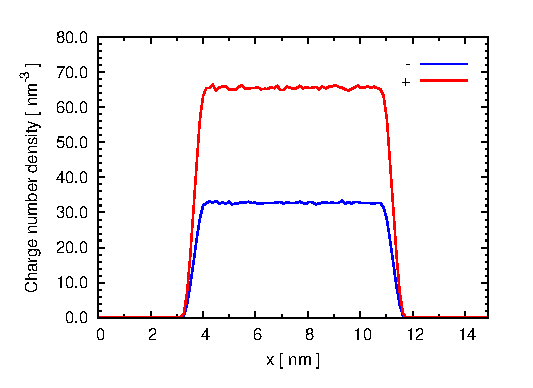
\includegraphics[]{rand1.rho.eps}
  \caption{
    The charge number density  of Example 2.
    The red line: positive charge. The blue line: negative charge.
    Since the charges are uniformly distributed
    on $y$ and $z$ direction, the densities are averaged on $y$ and $z$,
    and plotted as a
    function of $x$.
  }
  \label{fig:tmp-rho1}
\end{figure}

In this example,  41472 charges are put into a
$14.90\textsf{nm}\times 7.45\textsf{nm}\times 7.45\textsf{nm}$
periodic simulation box. One third of
them are carrying negative charge of $-0.834e$, and the other two thirds
are carrying positive charge of $+0.417e$.
The position of these charges
are randomly generated subjecting to the number density shown in
Fig.~\ref{fig:tmp-rho1}.  The number density of the  positive
charge   is twice as large as that of the negative charge,
so the
positive and negative charges cancel, and the
system is \emph{locally} neutral. Notice the amount of charges
and the density distributions are intentionally chosen the same as
Example 3~(see section \ref{sec:example3}), 
for an easy comparison.  The only difference is that the positions
of charges are independent  in this example,
while they are correlated in Example 3.
% Both the density distributions are highly
% inhomogeneous, take the positive distribution for example: between 11
% \textsf{nm} and 29 \textsf{nm}, the charge density is
% $1.0\;\textsf{e/nm}^3$, while between 0 \textsf{nm} to 9 \textsf{nm}
% and between 31 \textsf{nm} to 40 \textsf{nm}, the density is
% $0.05\;\textsf{e/nm}^3$.

% \begin{figure}
%   \centering
%   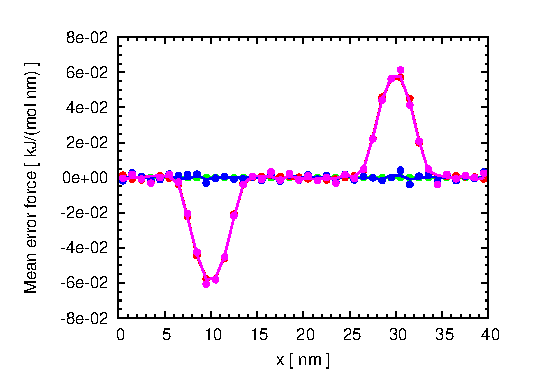
\includegraphics[]{fig/error.one_peak.box40x20x20.b1.000.r3.00.n6.K101x051x051/fig.ana.ewald.meanf.eps}
%   \caption{Example 1: the actual (denoted by dots) and estimated
%     (denoted by straight lines) mean error force of the direct part
%     $\langle\Delta \v F_{\textrm{dir}}\rangle$ (red), reciprocal
%     part of Ewald summation $\langle\Delta \v F_{\textrm{rec}}p\rangle$ (green) and the reciprocal part of the analytical
%     differentiation $\langle\Delta \v
%     F^{\textrm{ana}}_{\textrm{rec}}\rangle$ (blue). The total
%     mean error force of analytical differentiation $\langle\Delta \v
%     F^{\textrm{ana}}\rangle$ is given in pink.  Since the charge
%     distribution is uniform on the $y$ and $z$ direction, the $y$ and
%     $z$ dimension of the mean error force is averaged, and the errors
%     are plotted on $x$ direction.  The cut-off in the real space is 3
%     \textsf{nm}, the number of freedom in the reciprocal space is
%     $100\times 50\times 50$, the parameter $\beta$ is $1.0\;
%     \textsf{nm}^{-1}$ and the order of B-spline interpolation used for
%     the analytical differentiation is 6.}
%   \label{fig:meanf1}
% \end{figure}

% Fig.~\ref{fig:meanf1} presents the mean error force of the direct part
% $\langle\Delta \v F_{\textrm{dir}}\rangle$, reciprocal part of Ewald
% summation $\langle\Delta \v F_{\textrm{rec}}\rangle$ and the
% reciprocal part of the analytical differentiation $\langle\Delta \v
% F^{\textrm{ana}}_{\textrm{rec}}\rangle$. The total mean error force of
% analytical differentiation, which is simply $\langle\Delta \v
% F^{\textrm{ana}}\rangle = \langle\Delta \v F_{\textrm{dir}}\rangle +
% \langle\Delta \v F^{\textrm{ana}}_{\textrm{rec}}\rangle$, is also
% given.  The real and estimated mean error forces are denoted by dots
% and straight lines, respectively. All estimates are consistent very
% well with real errors.  Since the system is locally neutral, the first
% order charge distribution $\rho_q$ is naturally zero, therefore, by
% Eqn. \eqref{eqn:tmp10}, \eqref{eqn:tmp18} and \eqref{eqn:ana.meanf}, all
% the mean error forces should varnish. Numerical resutls in
% Fig. \ref{fig:meanf1} verifies with the above discussion.

\begin{figure}
  \centering
  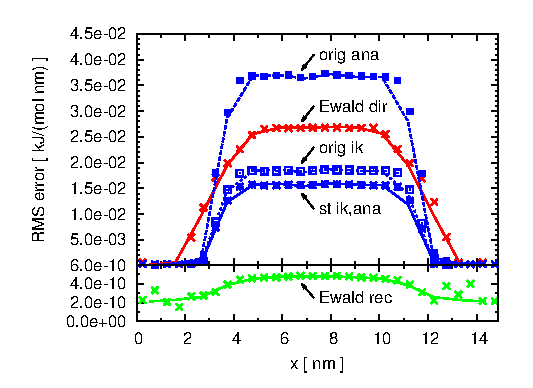
\includegraphics[]{fig.rand1.error.eps}
  \caption{
    Example 1: the real RMS errors and the corresponding
    estimates. Different colors denote
    different parts of the Ewald summation. Red: the direct
    part of Ewald summation. Green: the reciprocal
    part of Ewald summation, calculated by truncation.
    ``$\times$'' denotes the real error, and the solid line denotes
    the estimated error.
    Blue: the reciprocal part of Ewald summation, calculated
    by fast algorithms. ``$\blacksquare$'': real error of
    the original analytical
    differentiation. ``$\boxdot$'': real error of the original ik-differentiation.
    ``$\times$'': real error of the staggered mesh analytical differentiation.
    ``$+$'': real error of the staggered mesh ik-differentiation.
    Dashed line: estimated original analytical differentiation.
    Dotted line: estimated original ik-differentiation.
    Solid line: estimated staggered mesh ik-/analytical differentiation.
    The RMS errors are averaged over $y$ and $z$ directions, and are
    plotted against $x$ axis.
    The cut-off in the real space is 1.31 \textsf{nm}, the number of
    freedom in the reciprocal space is $120\times 60\times 60$, the
    parameter $\beta$ is $2.5\; \textsf{nm}^{-1}$, and the order of
    B-spline interpolation is 6.
    }
    % Example 1: the actual (denoted by dots) and estimated
    % (denoted by straight lines) RMS force error of the direct part
    % $\sqrt{\langle\vert\Delta \v F_{\textrm{dir}}\vert^2\rangle}$
    % (red), reciprocal part of Ewald summation
    % $\sqrt{\langle\vert\Delta \v F_{\textrm{rec}}\vert^2\rangle}$
    % (green) and the reciprocal part of the analytical differentiation
    % $\sqrt{\langle\vert\Delta \v
    %   F^{\textrm{ana}}_{\textrm{rec}}\vert^2\rangle}$ (blue). The RMS
    % force error of analytical differentiation
    % $\sqrt{\langle\vert\Delta \v F^{\textrm{ana}}\vert^2\rangle}$ is
    % given in pink.  Since the charge distribution is uniform on the
    % $y$ and $z$ direction, the $y$ and $z$ dimension of the mean error
    % force is averaged, and the errors are plotted on $x$ direction.
    % The cut-off in the real space is 3 \textsf{nm}, the number of
    % freedom in the reciprocal space is $100\times 50\times 50$, the
    % parameter $\beta$ is $1.0\; \textsf{nm}^{-1}$ and the order of
    % B-spline interpolation used for the analytical differentiation is
    % 6.}
  \label{fig:error1}
\end{figure}

Fig.~\ref{fig:error1} presents the real RMS error (by points) and the
corresponding error estimates (by lines) of the cut-offed Ewald direct
part, the truncated Ewald reciprocal part, the original ik-/analytical
differentiation and the staggered mesh ik-/analytical
differentiation. All the error estimates are consistent very well
with the real errors.  The parameters are
chosen to be the same for an easy comparison among the
reciprocal space methods.  The errors of FFT
based fast Ewald methods are 8 orders of magnitudes large than that of
the truncated Ewald summation.
This supports the argument addressed in
Sec.~\ref{sec:error-ik}: the error introduced by truncating the
reciprocal Ewald summation is much smaller than that introduced by
approximating $e^{2\pi i\v m\cdot\v r}$.
The original ik-differentiation is more accurate than
the original analytical differentiation.
With the staggered mesh,
the error of the analytical differentiation reduces by more than 50\%,
while the accuracy of the ik-differentiation is only marginally
improved.
The errors of the staggered mesh ik- and analytical differentiation
are identical, which supports the theoretical prediction.
The original ik-differentiation uses 4
FFT transforms, and the original analytical differentiation uses
only 2.  Therefore, the staggered mesh analytical differentiation uses
the same amount of FFTs as the original ik-differentiation, and saves
one half FFTs than the staggered mesh ik-differentiation.  As mentioned before,
the FFT is a bottleneck of communication on massive parallel
super-computers,
so the methods using less FFTs may have advantages on these machines.

% Fig.~\ref{fig:error1} presents the RMS force error of the direct part
% $\sqrt{\langle\vert\Delta \v F_{\textrm{dir}}\vert^2\rangle}$,
% reciprocal part of Ewald summation $\sqrt{\langle\vert\Delta \v
%   F_{\textrm{rec}}\vert^2\rangle}$, the reciprocal part of the
% analytical differentiation $\sqrt{\langle\vert\Delta \v
%   F^{\textrm{ana}}_{\textrm{rec}}\vert^2\rangle}$ and the total
% analytical differentiation force $\sqrt{\langle\vert\Delta \v
%   F^{\textrm{ana}}\vert^2\rangle}$.  The real and estimated mean error
% forces are denoted by dots and straight lines, respectively. All the
% error estimates are overlapping with the real errors, that means the
% error estimates developed by the present paper are very sharp.
% Since all mean error forces varnish, the RMS force errors
% consists of only the homogeneous contribution. 
% In the high charge density region, the error is comparatively larger
% than the low charge density region. For the direct part, the ratio is
% roughly the sqare root of the density ratio. For the reciprocal part
% this ratio is lower. The reciprocal error of the analytical
% differentiation is 4 orders of maganitudes large than that of the
% Ewald summation, which means the Ewald summation is much more precice
% than the fast algorithm based on mesh discretization.


% \begin{figure}
%   \centering
%   \includegraphics[width=.48\textwidth]{fig/error.one_peak.box40x20x20.b1.000.r3.00.n6.K101x051x051/fig.ik.meanf.eps}
%   \includegraphics[width=.48\textwidth]{fig/error.one_peak.box40x20x20.b1.000.r3.00.n6.K101x051x051/fig.ana.meanf.eps}
%   \caption{Resulting mean error force}
%   \label{fig:tmp1}
% \end{figure}

% \begin{figure}
%   \centering
%   \includegraphics[width=.48\textwidth]{fig/error.one_peak.box40x20x20.b1.000.r3.00.n6.K101x051x051/fig.ik.error.eps}
%   \includegraphics[width=.48\textwidth]{fig/error.one_peak.box40x20x20.b1.000.r3.00.n6.K101x051x051/fig.ana.error.eps}
%   \caption{Resulting RMS errors}
%   \label{fig:tmp2}
% \end{figure}

\subsection{Example 2: separated positive and negative charge}
\label{sec:example2}

\begin{figure}
  \centering
  % 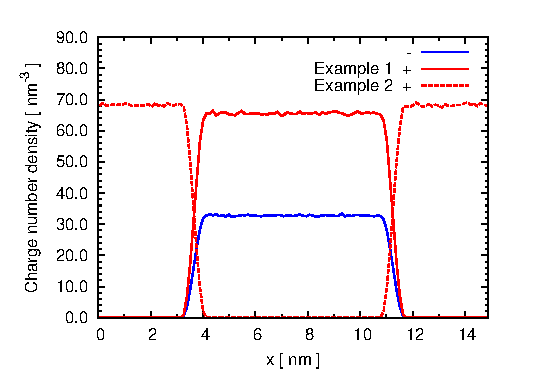
\includegraphics[width=.48\textwidth]{fig.new/rand2/fig.rho.eps}
  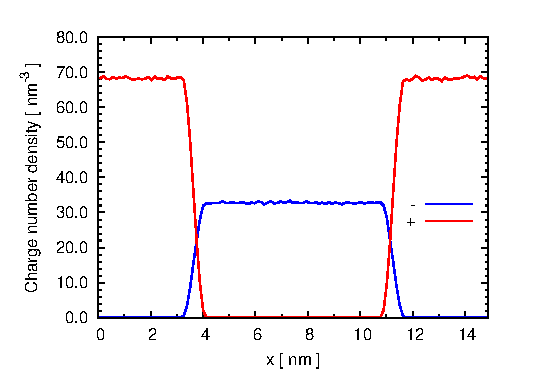
\includegraphics[]{rand2.rho.eps}
  \caption{Charge distribution of Example 2. The red line
    denotes the positive charge distribution, while the blue line
    denotes the negative charge distribution. Since all distributions
    are uniform on $y$ and $z$ direction, they are plotted as a
    function of $x$.}
  \label{fig:tmp-rho2}
\end{figure}

In this example, the setting is nearly the same as
Example 1. The only difference is that all positive charges
are moved to the region where the density of negative charge is low,
see Fig.~\ref{fig:tmp-rho2}.
In this system, the negative charges are separated from their
counter ions, but the whole system is kept neutral. This case rarely
happens in real simulation, but it serves as a good test of the error
estimates in extreme situations.

\begin{figure}
  \centering
  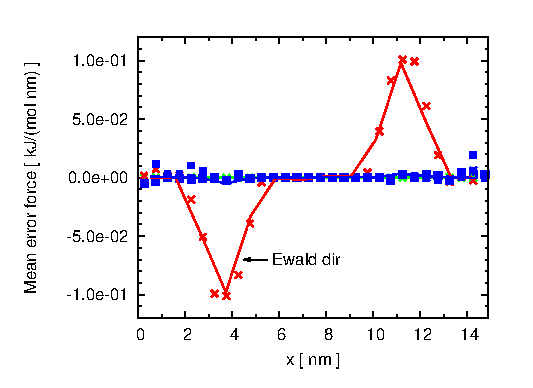
\includegraphics[]{fig.rand2.meanf.eps}
  \caption{
    Example 2: the real mean error forces and the corresponding
    estimates. All symbols and working parameters are the same
    as     Fig.~\ref{fig:error1}.
    The reciprocal mean error forces vanish, so the points and lines
    overlap each other. 
    The errors are averaged over $y$ and $z$ directions, and are
    plotted against $x$ axis.
    % Red: the direct
    % part of Ewald summation. Green: the reciprocal
    % part of Ewald summation, calculated by truncation.
    % ``$\times$'' denotes the real error, and the solid line denotes
    % the estimated error.
    % Blue: the reciprocal part of Ewald summation, calculated
    % by fast algorithms. ``$\blacksquare$'': real error of
    % the oringinal analytical
    % differentiation. 
    % ``$\times$'': real error of the staggered mesh analytical differentiation.
    % Dashed line: estimated oringinal analytical differentiation.
    % Solid line: estimated staggered mesh ik-/analytical differentiation.
    % The $x$ component of the
    % error forces are averged over $y$ and $z$ directions, and are
    % plotted against $x$ axis.
    % The cut-off in the real space is 1.31 \textsf{nm}, the number of
    % freedom in the reciprocal space is $120\times 60\times 60$, the
    % parameter $\beta$ is $2.5\; \textsf{nm}^{-1}$, and the order of
    % B-spline interpolation is 6.
    }
  \label{fig:meanf2}
\end{figure}


Fig.~\ref{fig:meanf2} shows the real mean error forces (by points) and the
corresponding error estimates (by lines) of cut-offed Ewald direct
part, truncated Ewald reciprocal part, the ik-/analytical
differentiation 
and the staggered mesh ik-/analytical differentiation. All
notations in the figure are the same as Example 1.  Although the
charge distribution is not usual in this case, the error estimates are still
sharp. The two peaks of the direct mean  error force present at the
positive-negative interface, due to the separation of the positive
and negative charges, i.e., a non-vanishing and fast changing first order charge
distribution $\rho_q$.  Similar phenomena was reported by
Ref.~\cite{wang2012}. Surprisingly, 
the reciprocal mean error forces
do not present any singularity, and varnish
all over the simulation region.

\begin{figure}
  \centering
  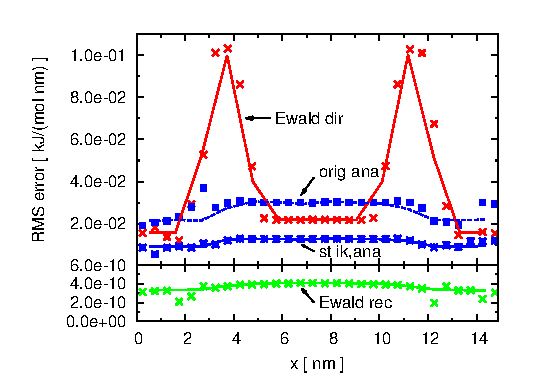
\includegraphics[]{fig.rand2.error.eps}
  \caption{
    Example 2: the real RMS error and the corresponding
    estimates.
    The symbols and working parameters used in this figure are the same as
    Fig.~\ref{fig:error1}.
    The real and estimated error of the original ik-differentiation
    are very closed to the staggered mesh Ewald results, so
    they are not shown in this figure for clarity, 
    The errors are averaged over $y$ and $z$ directions, and are
    plotted against $x$ axis.
  }
  \label{fig:error2}
\end{figure}

Fig.~\ref{fig:error2} presents the real and estimated
RMS error of Example 2. The
the original ik-differentiation is not
shown, because it is nearly indistinguishable from the staggered
mesh ik-/analytical differentiation in this plot.
All the error estimates consist with the real errors.
Stemming from the inhomogeneity error,
two peaks of the direct error form at the interfacial
regions, and are much larger than the error in bulk
regions~\cite{wang2012}.
The reciprocal RMS errors only contain homogeneity contributions,
due to the varnished mean error force.
Similar with Example 1, the truncated Ewald
method is much more precise than the fast algorithms, and the
staggered mesh improves the accuracy of analytical
differentiation by more than 50\%.


% Fig. \ref{fig:error2} shows the RMS errors of Example 2. The
% corresponding error estimates are accurate. In this case the second
% order charge distrubution is a constant, therefore the contribution to
% the error is also a constant. The same as Example 1, the reciprocal
% error of Ewald sum is much smaller than the direct error and the
% reciprocal error of analytical differentiation.  The error peak at the
% positive-negative interface, is only 3 times larger than the error of
% the bulk regions. For the dispersion interaction, the interfacial
% error could be more than one order of maganitude larger than the bulk
% error. That is because the direct interaction converges much faster
% than the dispersion interaciton ($e^{-r^2}$ v.s. $r^{-6}$).

% \begin{figure}
%   \centering
%   \includegraphics[width=.48\textwidth]{fig/error.two_peaks_sep.box40x20x20.b1.000.r3.00.n6.K101x051x051/fig.ik.meanf.eps}
%   \includegraphics[width=.48\textwidth]{fig/error.two_peaks_sep.box40x20x20.b1.000.r3.00.n6.K101x051x051/fig.ana.meanf.eps}
%   \caption{Resulting mean error force}
%   \label{fig:tmp3}
% \end{figure}

% \begin{figure}
%   \centering
%   \includegraphics[width=.48\textwidth]{fig/error.two_peaks_sep.box40x20x20.b1.000.r3.00.n6.K101x051x051/fig.ik.error.eps}
%   \includegraphics[width=.48\textwidth]{fig/error.two_peaks_sep.box40x20x20.b1.000.r3.00.n6.K101x051x051/fig.ana.error.eps}
%   \caption{Resulting RMS errors}
%   \label{fig:tmp4}
% \end{figure}

\subsection{Example 3: a water system in gas-liquid phase equilibrium}
\label{sec:example3}

This example studies the gas-liquid phase equilibrium of a water
system. The size of the simulation box and number of charges are the
same as Example 1 (Sec.~\ref{sec:example1}): 13824 TIP3P water
molecules~\cite{jorgensen1983comparison} are put into a
$14.90\textsf{nm}\times 7.45\textsf{nm}\times 7.45\textsf{nm}$
periodic simulation box.  The molecules dynamics simulations of this
system was performed by GROMACS 4.5~\cite{hess2008gromacs}.  The system
is coupled to a velocity rescale thermostat~\cite{bussi2007canonical}
at temperature 300~\textsf{K}, and simulated long enough to reach the
equilibrium. After the equilibrium,
the water molecules separate into the liquid and vapor phases.
The number densities of oxygen and hydrogen atoms
are the same as those shown by Fig.~\ref{fig:tmp-rho1}.
50 consequential snapshots of
the system are taken along the MD trajectory
with a time interval of 20~\textsf{ps}.  These
snapshots are used to calculate the real error and the charge densities
for the error estimates.

\begin{figure}
  \centering
  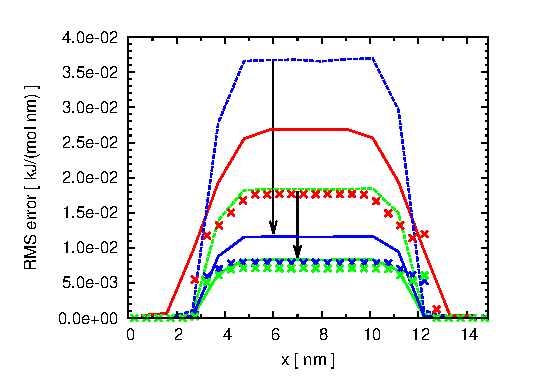
\includegraphics[]{fig.water.orig.error.eps}
  \caption{
    Example 3: the real RMS errors and the corresponding
    estimates of original ik- and analytical differentiation.
    Red: the direct part.
    Green: the original ik-differentiation.
    Blue: the original analytical differentiation.
    ``$\times$'': the real error.
    Dashed line: the error estimate, without the correlation error estimate.
    Solid  line: the error estimate, with the nearest neighbor
    approximation of the correlation error.
    The working parameters are the same as Example 1.
    The black arrows indicate the improvement
    of error estimate by including nearest neighbor
    approximation of correlation error.
  }   
  \label{fig:water-error0}
\end{figure}

\begin{figure}
  \centering
  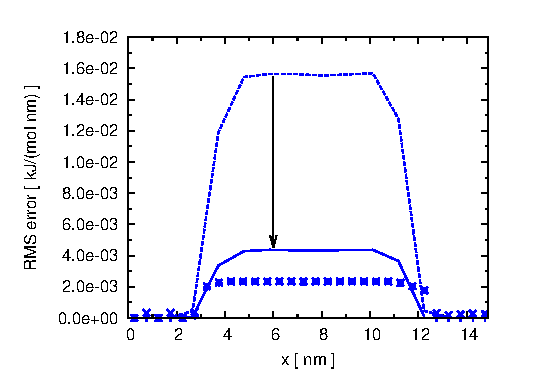
\includegraphics[]{fig.water.ana.st.error.eps}
  \caption{
    Example 3: the real RMS errors and the corresponding
    estimates. 
    Blue ``$\times$'': the real error of the staggered mesh
    analytical differentiation.
    Blue ``$+$'': the real error of the staggered mesh
    ik-differentiation, it is overlapping with the analytical differentiation.
    Blue dashed line: the error estimate, without the correlation error.
    Blue solid line: the error estimate, with the nearest
    neighbor approximation of the correlation error.
    The RMS errors are averaged over $y$ and $z$ directions, and are
    plotted against $x$ axis.
    The working parameters are the same as Example 1.
    The black arrow indicates the improvement
    of error estimate by including nearest neighbor
    approximation of correlation error.
  }   
  \label{fig:water-error}
\end{figure}

The real and estimated errors of the original SPME
(both ik- and analytical differentiation)
and the staggered mesh Ewald (both ik- and analytical differentiation)
are in Fig.~\ref{fig:water-error0}
and Fig.~\ref{fig:water-error}, respectively.
Unlike previous examples, the real error of ik- and analytical differentiation
are nearly the same.
The staggered mesh ik- and analytical differentiation
are also equivalent in this case, and are $\sim$70\% more accurate
than the original ik-/analytical differentiation.
In this case,
all estimates without considering the correlation error
deviate from the real errors.
The quality of the direct
part errors estimates is still good (though not perfect):
the error is overestimated by~50\%.
The RMS errors of the ik-differentiation, analytical differentiation
and the staggered mesh ik-/analytical differentiation are
overestimated by 2.6, 4.7 and 6.8 times, respectively.
Notice the only difference between this example
and Example 1 (in which the estimates were very sharp) is the correlation
of the charges in the system,
which plays a very important role in the RMS error. 
More surprisingly, the correlation
actually  reduces the error in the force computation.
Currently we have no explanation for this phenomena.
% Anyway, the correlation error $\mathcal
% E_{\textrm{correlation}}$ should be included to develop a more accurate error
% estimate. 
By including the nearest neighbor approximation of the
correlation error, the quality of all error estimates is improved greatly,
as indicated by the arrows in Fig.~\ref{fig:water-error0} and \ref{fig:water-error}.
Now the RMS errors of ik-differentiation, analytical differentiation
and staggered mesh ik-/analytical differentiation
are overestimated by a factor of 1.16, 1.44 and 1.86,
respectively.
Ref.~\cite{wang2010optimizing} showed that the error estimate
(ik-differentiation in a homogeneous water system) that
is even three times larger than the real error
still works well in the parameter tuning process, 
so the error estimate for  all methods are now good enough
for the parameter tuning application.
The great improvement by the nearest neighbor approximation 
means that  among all atomic
correlates (i.e. the rigid H-O bond and H-O-H angle, the van der Waals interactions,
the hydrogen bonds, etc.), the rigid bond and angle correlation
% (rigid
% modeling of H-O bond and H-O-H angle)
is the most important one, and all
the rest account for the remaining discrepancy between the estimated and real
error.


% pbut the error
% estimate for the analytical differentiation is problematic.
% The error estimate of the staggered mesh analytical differentiation is 6.8 times
% larger than the real error,
% which means the
% positional correlation of charges plays a very important role
% in the error estimate. More surprisingly, the correlation
% actually greatly reduces the error in force computation.
% Currently we have no explaination for this phenomenon.
% Anyway, the correlation error $\mathcal
% E_{\textrm{correlation}}$ should be included to develop a more accurate error
% estimate. 
% By including the first neighbor approximation of the
% correlation error, the error estimate is imporved greatly
% (as indicated by the arrow in Fig.~\ref{fig:water-error}), and is only
% twice as large as the real error.
% This means among all atomic
% correlates (i.e. the chemical bonds, the van der Waals interactions,
% the hydrogen bonds, etc.), the first neighbor correlation (chemical bond)
% is the most important one, and all
% the rest account for the remaining discrepancy between the estimated and real
% error.
% The error estimate for staggered mesh Ewald is now good enough
% for the parameter tuning application.
% In this example, although both error estimates are
% not as sharp as the uncorrelated examples (Example 1 \& 2), they are
% good enough to derive for the parameter
% optimization~\cite{wang2010optimizing}.

\section{Conclusions and remarks}
\label{sec:conclusions}

In this paper, we proposed the error estimates for three state-of-art
algorithms calculating the long-range electrostatic interaction in a
molecular system. They were the Ewald summation, the smooth particle
mesh Ewald (SPME, both ik- and analytical differentiation) and
the staggered mesh Ewald (both ik- and analytical differentiation) methods.
Unlike the previous error estimates, the new error estimates did NOT
assume the homogeneity and uncorrelation of the system, which was a too
strong assumption for most molecular simulations of practical
interest.  A general error estimate framework was proposed
to study all the aforementioned estimates.
When the error force has a pairwise form,
the RMS error was proved to be composed by three additive parts:
the homogeneity error, the inhomogeneity error and the correlation
error.
Moreover, the framework quantitatively provided the estimate
of all these error components, and suggested a computationally
scalable way (at the cost of $\mathcal O(N\log N)$) to calculate them.

% the estimates for all these error 
% were easily derived by the proposed framework.

% by
% which the RMS error was proved to be composed by three additive parts:
% the homogeneity error, the inhomogeneity error and the correlation
% error.

% The homogeneity and inhomogeneity error estimates are
% computationally feasible 
% only when they can be written in a
% convolution form.  The correlation error that is a twofold
% convolution was approximated by the nearest neighbor approximation, in
% order to reduce the computational cost to $\mathcal O(N\log N)$.


% The correlation of the charges is considered by the nearest
% neighbor approximation, which greatly
% improved the qulity of the error estimate in the water system.

Some minor contributions of the present work are:
\begin{itemize}\itemsep -3pt
\item In a locally neutral charge system, the inhomogeneity
  error was proved to vanish. Therefore, the error
  is of good property, and no adaptive method nor
  force correction~\cite{wang2012} is necessary. Fortunately, most
  molecular systems of practical interests are locally neutral.
\item We explicitly gave the expression of the self-interaction term
  in the analytical differentiation, which was proved to dominant the
  force error in low density systems~\cite{cerutti2009staggered}.  The
  expression helped removing the self-interaction term at a very low
  computational cost.
\item The error estimate showed that the staggered mesh Ewald
  (both ik- and analytical differentiation) are always more precise than
  the original SPME.
\item Unlike the original analytical differentiation
  that violates the Newton's third law, the staggered mesh analytical
  differentiation preserves it to the leading order.
\item We also proved the equivalence of the staggered mesh ik- and analytical
  differentiation, to the leading order of the force error.
  The staggered mesh analytical differentiation requires only one half
  FFTs as the ik-differentiation, so the former may be preferable
  for massive parallel simulation, due to the bottleneck of all-to-all
  communication required by the parallel FFT.
\end{itemize}

The effectiveness of the proposed error estimates was verified by
three numerical tests: two ideal inhomogeneous cases, in which the charges
were uncorrelated,
and one real water system, in which the charges were correlated.
In the ideal cases, the all error estimates were sharp, even in an extreme
case: positive and negative charges were globally separated. 
In the water system,  all estimates overestimated the real error,
because of the correlation of charges.
The quality of the real space error estimates 
was acceptable.
% However, the error estimate neglecting the charge correlation
% is not applicable  for the staggered mesh Ewald method.
The error estimates for the reciprocal space fast algorithms
were impressively improved by including the first neighbor approximation
to the correlation error.
This indicated among all possible correlations,
the rigid bond and angle correlation within one molecule
was dominant.

This paper only focuses on the accuracy of the
mentioned long-range algorithms.
We do not touch the topic of comparing the efficiency of these algorithms.
To be fair,
we propose 
optimizing the working parameters for each algorithm with a
predetermined accuracy before
comparing
the real execution speed.
Such a comparison includes the topic of the hardware architecture,
the communication bandwidth,
the software implementation, the scalability of the problem,
the inhomogeneity of the system, etc..
They are far beyond the scope of the current
work, and will be discuss in the following research.




\appendix
\section{Error estimate of the smooth particle mesh
Ewald method}
\label{sec:appendix}

\subsection{ik-differentiation}
Starting from Eqn.~\eqref{eqn:ik.error.force}, we have the error force kernel
of the ik-differentiation:
\begin{align}
  \v K^{\textrm{ik}}_{\textrm{rec}}(\v r, \v r')
  =
  \sum_{
    \begin{subarray}{c}
      \vert m_{\alpha}\vert < K_\alpha/2\\
      \v m\neq 0
    \end{subarray}}
  [\,A(\v m, \v r) + A(\v m,-\v r')\,]
  \v g(\v m)\,e^{-2\pi i\v m\cdot(\v r-\v r')}
\end{align}
By inserting Eqn.~\eqref{eqn:error-A}, the error force kernel is
\begin{align}
  \label{eqn:ik.kernel.2}
  \v K^{\textrm{ik}}_{\textrm{rec}}(\v r, \v r')
  =
  \sum_{
    \begin{subarray}{c}
      \vert m_{\alpha}\vert < K_\alpha/2\\
      \v m\neq 0
    \end{subarray}}
  \sum_{\alpha=1}^3\sum_{l\neq 0}
  \,(
  e^{2\pi i l K_\alpha\v a^\ast_\alpha\cdot \v r} +
  e^{-2\pi i l K_\alpha\v a^\ast_\alpha\cdot \v r'}
  - 2
  )
  Z_{\alpha,l}(\v m)
  \v g(\v m)\,e^{-2\pi i\v m\cdot(\v r-\v r')}
\end{align}
To calculate the mean error force estimate, we should
calculate the integral of
$\int \v K^{\textrm{ik}}_{\textrm{rec}}(\v r, \v r')\rho_q(\v r')\,\d d\v r$.
By Eqn.~\eqref{eqn:ik.kernel.2}, we should calculate
$  \int e^{-2\pi i l K_\alpha\v a^\ast_\alpha\cdot \v r'}\rho_q(\v r')
\,e^{2\pi i\v m\cdot\v r'}\,\d d\v r'$, which is the inverse Fourier transform
of $e^{-2\pi i l K_\alpha\v a^\ast_\alpha\cdot \v r'}\rho_q(\v r')$. Notice,
for example, when $\alpha=1$ we have:
\begin{align}
  [\,\rho_q(\v r')\,e^{-2\pi i l K_1\v a^\ast_1\cdot \v r'}\,] ^\vee
  (m_1, m_2, m_3)
  = \check\rho(m_1-lK_1, m_2, m_3).
\end{align}
Since $\vert m_1\vert < K_1/2$ and $l\neq 0$,
$\check\rho(m_1-lK_1, m_2, m_3)$ is
the high wave number (higher than $K_\alpha / 2$) part of the density profile.
If the density is smooth enough, this term can be reasonably neglected.
Therefore,
\begin{align}\nonumber
  \langle\Delta\v F^{\textrm{ik}}_{\textrm{rec}}(\v r)\rangle
  =\,&
  q\, \int_{\mathbb R^3}
  \v K^{\textrm{ik}}_{\textrm{rec}} (\v r,\v r')\,\rho_q(\v r')\,\d d\v r'\\
  \approx\,&
  q
  \big\{
  \big[
  \sum_{\alpha}\sum_{l\neq 0}
  (e^{2\pi i l K_\alpha\v a^\ast_\alpha\cdot \v r}   - 2 )
  \v G_{\alpha,l}
  \big]
  \ast\rho_q\,
  \big\} (\v r),
\end{align}
Further neglecting the
high-wave-number term $e^{2\pi i l K_\alpha\v a^\ast_\alpha\cdot \v r}$, we reach:
\begin{align}
  \langle\Delta\v F^{\textrm{ik}}_{\textrm{rec}}(\v r)\rangle
  \approx\,&
  -2q
  \big[
  \big(
  \sum_{\alpha}\sum_{l\neq 0}\v G_{\alpha,l}
  \big)
  \ast\rho_q\,
  \big] (\v r).
\end{align}

To calculate the RMS error, we square the error force kernel:
\begin{align}\nonumber
  \vert\v K^{\textrm{ik}}_{\textrm{rec}}(\v r,\v r')\vert^2
  =\,&
  \sum_{
    \begin{subarray}{c}
      \vert m_{\alpha}\vert < K_\alpha/2\\
      \v m\neq 0
    \end{subarray}}
  \sum_{
    \begin{subarray}{c}
      \vert n_{\alpha}\vert < K_\alpha/2\\
      \v n\neq 0
    \end{subarray}}
  \sum_{\alpha,\beta}
  \sum_{l_1,l_2}
  \v g(\v m)\cdot\v g(\v n)\,
  Z_{\alpha,l_1}(\v m)Z_{\beta,l_2}(\v n)
  \\\nonumber
  &\,
  \times
  \,(
  e^{2\pi i l_1 K_\alpha\v a^\ast_\alpha\cdot \v r} +
  e^{-2\pi i l_1 K_\alpha\v a^\ast_\alpha\cdot \v r'}
  - 2
  )
  \,(
  e^{-2\pi i l_2 K_\beta\v a^\ast_\beta\cdot \v r} +
  e^{2\pi i l_2 K_\beta\v a^\ast_\beta\cdot \v r'}
  - 2
  )\\
  &\,
  \times
  e^{-2\pi i(\v m-\v n)\cdot(\v r-\v r')}
\end{align}
By  carefully calculating
$  (
e^{2\pi i l_1 K_\alpha\v a^\ast_\alpha\cdot \v r} +
e^{-2\pi i l_1 K_\alpha\v a^\ast_\alpha\cdot \v r'}
- 2
)
\,(
e^{-2\pi i l_2 K_\beta\v a^\ast_\beta\cdot \v r} +
e^{2\pi i l_2 K_\beta\v a^\ast_\beta\cdot \v r'}
- 2
)$:
\begin{align}\nonumber
  &(
  e^{2\pi i l_1 K_\alpha\v a^\ast_\alpha\cdot \v r} +
  e^{-2\pi i l_1 K_\alpha\v a^\ast_\alpha\cdot \v r'}
  - 2
  )
  \,(
  e^{-2\pi i l_2 K_\beta\v a^\ast_\beta\cdot \v r} +
  e^{2\pi i l_2 K_\beta\v a^\ast_\beta\cdot \v r'}
  - 2
  ) \\ \nonumber
  = \,&
  e^{2\pi i(l_1K_\alpha\v a^\ast_\alpha - l_2K_\beta\v a^\ast_\beta)\cdot\v r} +
  e^{-2\pi i(l_1K_\alpha\v a^\ast_\alpha - l_2K_\beta\v a^\ast_\beta)\cdot\v r'} \\
  \label{eqn:ik.cal.tmp1}
  &-2(
  e^{2\pi i l_1 K_\alpha\v a^\ast_\alpha\cdot \v r} +
  e^{-2\pi i l_1 K_\alpha\v a^\ast_\alpha\cdot \v r'}
  ) 
  -2(
  e^{2\pi i l_1 K_\alpha\v a^\ast_\alpha\cdot \v r} +
  e^{-2\pi i l_1 K_\alpha\v a^\ast_\alpha\cdot \v r'}
  ) + 4
\end{align}
The first two term on the r.h.s. of Eqn.~\eqref{eqn:ik.cal.tmp1}
are not high-wave-number terms only when $l_1 = l_2$ and $\alpha=\beta$.
The third and fourth terms are always high-wave-number terms,
because $l_1\neq 0$ and $l_2\neq 0$.
Therefore, we have the error estimate
for the RMS homogeneity error:
\begin{align}\nonumber
  [\mathcal E^{\textrm{ik}}_{\textrm{homo}}(\v r)]^2
  = \,&
  \int
  \vert\v K^{\textrm{ik}}_{\textrm{rec}}(\v r,\v r')\vert^2
  \rho_{q^2}(\v r')\,\d d\v r' \\
  \approx\,&  
  2q^2
  \big[\,
  \big(
  \sum_{\alpha} \sum_{l\neq 0}
  \vert \v G_{\alpha,l}\vert^2
  \big)
  \ast \rho_{q^2}
  \,\big] (\v r)
  +
  4q^2\,
  \big[
  \vert
  \sum_{\alpha} \sum_{l\neq 0}  
  \v G_{\alpha,l}
  \vert^2
  \ast \rho_{q^2}\,
  \big] (\v r) 
\end{align}

It is also possible to calculate the first neighbor approximation for the
ik-differentiation. Firstly, we have:
\begin{align}\nonumber
  \big\langle
  \v K^{\textrm{ik}}_{\textrm{rec}}(\v r, \v r'+\v s)
  \big\rangle
  = \,&
  \sum_{
    \begin{subarray}{c}
      \vert m_{\alpha}\vert < K_\alpha/2\\
      \v m\neq 0
    \end{subarray}}
  \sum_{\alpha=1}^3\sum_{l\neq 0}
  Z_{\alpha,l}(\v m)
  \v g(\v m) \\ \nonumber
  \,&
  \times
  \big\langle
  (
  e^{2\pi i l K_\alpha\v a^\ast_\alpha\cdot \v r} +
  e^{-2\pi i l K_\alpha\v a^\ast_\alpha\cdot (\v r' + \v s)}
  - 2
  )\,
  e^{-2\pi i\v m\cdot(\v r-\v r' -\v s)}
  \big\rangle \\
  \approx\,&
  \sum_{
    \begin{subarray}{c}
      \vert m_{\alpha}\vert < K_\alpha/2\\
      \v m\neq 0
    \end{subarray}}
  \sum_{\alpha=1}^3\sum_{l\neq 0}
  (
  e^{2\pi i l K_\alpha\v a^\ast_\alpha\cdot \v r} 
  - 2
  )\,
  Z_{\alpha,l}(\v m)
  \v g(\v m)
  \hat T_s(\v m)
  e^{-2\pi i\v m\cdot(\v r-\v r')}  
\end{align}
So
\begin{align}\nonumber
  \v K^{\textrm{ik}}_{\textrm{rec}}(\v r,\v r')\cdot
  \big\langle
  \v K^{\textrm{ik}}_{\textrm{rec}}(\v r, \v r'+\v s)
  \big\rangle
  =\,&
  \sum_{
    \begin{subarray}{c}
      \vert m_{\alpha}\vert < K_\alpha/2\\
      \v m\neq 0
    \end{subarray}}
  \sum_{
    \begin{subarray}{c}
      \vert n_{\alpha}\vert < K_\alpha/2\\
      \v n\neq 0
    \end{subarray}}
  \sum_{\alpha,\beta}
  \sum_{l_1,l_2}
  \v g(\v m)\cdot\v g(\v n)\,
  Z_{\alpha,l_1}(\v m)Z_{\beta,l_2}(\v n)\hat T_s(\v n)
  \\\nonumber
  &\,
  \times
  \,(
  e^{2\pi i l_1 K_\alpha\v a^\ast_\alpha\cdot \v r} +
  e^{-2\pi i l_1 K_\alpha\v a^\ast_\alpha\cdot \v r'}
  - 2
  )
  \,(
  e^{-2\pi i l_2 K_\beta\v a^\ast_\beta\cdot \v r}
  - 2
  )\\
  &\,
  \times
  e^{-2\pi i(\v m-\v n)\cdot(\v r-\v r')}
\end{align}
Inserting it into Eqn.~\eqref{eqn:c-error-1}, also neglect the high
frequency terms yields
% \begin{align}
%   q^2 q_{\textrm{H}}
%   \int
%   \v K^{\textrm{ik}}_{\textrm{rec}}(\v r,\v r)\cdot
%   \big\langle
%   \v K^{\textrm{ik}}_{\textrm{rec}}(\v r, \v r+\v s)
%   \big\rangle\,\rho_{\textrm{O}}(\v r)\,
%   \d d\v r
% \end{align}
\begin{align}\nonumber
  \mathcal E^{\textrm{ik}}_{\textrm{correlation}}(\v r)
  =\,&
  q^2
  \big[\,
  \big(
  \sum_{\alpha} \sum_{l\neq 0}
  \v G_{\alpha,l}\cdot[\hat T_{\textrm{O}}\hat{\v G}_{\alpha,l}]^{\vee}
  \big)
  \ast \rho_{\textrm{O}}
  \,\big] (\v r) \\\nonumber
  \,&+
  4q^2\,
  \big[
  \big(
  \sum_{\alpha} \sum_{l\neq 0}  
  \v G_{\alpha,l}
  \big)
  \cdot
  \big(
  \sum_{\alpha} \sum_{l\neq 0}  
  [\,\hat T_{\textrm{O}}\hat{\v G}_{\alpha,l}]^{\vee}
  \big)
  \ast \rho_{\textrm{O}}\,
  \big] (\v r) \\\nonumber
  \,&+
  q^2
  \big[\,
  \big(
  \sum_{\alpha} \sum_{l\neq 0}
  \v G_{\alpha,l}\cdot[\hat T_{\textrm{H}}\hat{\v G}_{\alpha,l}]^{\vee}
  \big)
  \ast \rho_{\textrm{H}}
  \,\big] (\v r) \\
  \,&+
  4q^2\,
  \big[
  \big(
  \sum_{\alpha} \sum_{l\neq 0}  
  \v G_{\alpha,l}
  \big)
  \cdot
  \big(
  \sum_{\alpha} \sum_{l\neq 0}  
  [\,\hat T_{\textrm{H}}\hat{\v G}_{\alpha,l}]^{\vee}
  \big)
  \ast \rho_{\textrm{H}}\,
  \big] (\v r) 
\end{align}


\subsection{analytical differentiation}
Starting from Eqn.~\eqref{eqn:ana.error.force}, we have the error force kernel
of the analytical differentiation (notice the self-interacting term is removed):
\begin{align}
  \v K^{\textrm{ana}}_{\textrm{rec}}(\v r, \v r')
  =
  \sum_{
    \begin{subarray}{c}
      \vert m_{\alpha}\vert < K_\alpha/2\\
      \v m\neq 0
    \end{subarray}}
  \{
  [A(\v m, \v r) + A(\v m,-\v r')\,]
  \v g(\v m) -
  2\v B(\v m,\v r) f(\v m)
  \}
  e^{-2\pi i\v m\cdot(\v r-\v r')}
\end{align}
By inserting Eqn.~\eqref{eqn:error-A} and \eqref{eqn:error-B}, we have
\begin{align}\nonumber
  \v K^{\textrm{ana}}_{\textrm{rec}}(\v r, \v r')
  =\,&
  \sum_{
    \begin{subarray}{c}
      \vert m_{\alpha}\vert < K_\alpha/2\\
      \v m\neq 0
    \end{subarray}}
  \sum_{\alpha=1}^3\sum_{l\neq 0}
  \big[
  \,(
  e^{2\pi i l K_\alpha\v a^\ast_\alpha\cdot \v r} +
  e^{-2\pi i l K_\alpha\v a^\ast_\alpha\cdot \v r'}
  - 2
  )
  \v g(\v m)
  \\ 
  \,&
  - 4\pi i l K_\alpha\v a_\alpha^\ast e^{2\pi i l K_\alpha\v a^\ast_\alpha\cdot \v r}
  f(\v m)
  \big]
  Z_{\alpha,l}(\v m)
  e^{-2\pi i\v m\cdot(\v r-\v r')}  
\end{align}
Following  the same idea as the error estimate of  ik-differentiation,
\begin{align}
  \langle\Delta\v F^{\textrm{ana}}_{\textrm{rec}}(\v r)\rangle
  \approx\,&
  -2q
  \big[
  \big(
  \sum_{\alpha}\sum_{l\neq 0}\v G_{\alpha,l}
  \big)
  \ast\rho_q\,
  \big] (\v r).
\end{align}
To calculate the RMS error, we start from
\begin{align}
  \vert\v K^{\textrm{ana}}_{\textrm{rec}}(\v r,\v r')\vert^2
  =\,&
  \sum_{
    \begin{subarray}{c}
      \vert m_{\alpha}\vert < K_\alpha/2\\
      \v m\neq 0
    \end{subarray}}
  \sum_{
    \begin{subarray}{c}
      \vert n_{\alpha}\vert < K_\alpha/2\\
      \v n\neq 0
    \end{subarray}}
  \sum_{\alpha,\beta}
  \sum_{l_1,l_2}
  \\\nonumber
  &\,
  \big[
  \,(
  e^{2\pi i l_1 K_\alpha\v a^\ast_\alpha\cdot \v r} +
  e^{-2\pi i l_1 K_\alpha\v a^\ast_\alpha\cdot \v r'}
  - 2
  )
  \v g(\v m)
  - 4\pi i l_1 K_\alpha\v a_\alpha^\ast e^{2\pi i l_1 K_\alpha\v a^\ast_\alpha\cdot \v r}
  f(\v m)
  \big] \\\nonumber
  \,&
  \times
  \big[
  \,(
  e^{2\pi i l_2 K_\beta\v a^\ast_\beta\cdot \v r} +
  e^{-2\pi i l_2 K_\beta\v a^\ast_\beta\cdot \v r'}
  - 2
  )
  \v g(\v n)
  - 4\pi i l_2 K_\beta\v a_\beta^\ast e^{2\pi i l_2 K_\beta\v a^\ast_\beta\cdot \v r}
  f(\v n)
  \big]
  \\
  &\,
  \times
  Z_{\alpha,l_1}(\v m)Z_{\beta,l_2}(\v n)
  e^{-2\pi i(\v m-\v n)\cdot(\v r-\v r')}
\end{align}
Similar to the calculation of \eqref{eqn:ik.cal.tmp1}, one can eventually
prove the error estimate for the homogeneity RMS error:
\begin{align}\nonumber
  [\mathcal E^{\textrm{ana}}_{\textrm{homo}}(\v r)]^2
  = \,&
  \int
  \vert\v K^{\textrm{ana}}_{\textrm{rec}}(\v r,\v r')\vert^2
  \rho_{q^2}(\v r')\,\d d\v r' \\\nonumber
  \approx\,&  
  q^2
  \big[\,
  \big(
  \sum_{\alpha} \sum_{l\neq 0}
  \vert \v G_{\alpha,l}\vert^2
  \big)
  \ast \rho_{q^2}
  \,\big] (\v r) +
  q^2
  \big[\,
  \big(
  \sum_{\alpha} \sum_{l\neq 0}
  \vert \v G_{\alpha,l} +\v F_{\alpha,l}\vert^2
  \big)
  \ast \rho_{q^2}
  \,\big] (\v r) \\
  \,&+
  4q^2\,
  \big[
  \vert
  \sum_{\alpha} \sum_{l\neq 0}  
  \v G_{\alpha,l}
  \vert^2
  \ast \rho_{q^2}\,
  \big] (\v r) 
\end{align}

To calculate the first neighbor approximation to the correlation error, 
\begin{align}\nonumber
  \big\langle
  \v K^{\textrm{ana}}_{\textrm{rec}}(\v r, \v r' + \v s)
  \big\rangle
  =\,&
  \sum_{
    \begin{subarray}{c}
      \vert m_{\alpha}\vert < K_\alpha/2\\
      \v m\neq 0
    \end{subarray}}
  \sum_{\alpha=1}^3\sum_{l\neq 0}
  \bigg\langle
  \big[
  \,(
  e^{2\pi i l K_\alpha\v a^\ast_\alpha\cdot \v r} +
  e^{-2\pi i l K_\alpha\v a^\ast_\alpha\cdot (\v r' + \v s)}
  - 2
  )
  \v g(\v m)
  \\\nonumber
  \,&
  - 4\pi i l K_\alpha\v a_\alpha^\ast e^{2\pi i l K_\alpha\v a^\ast_\alpha\cdot \v r}
  f(\v m)
  \big]
  Z_{\alpha,l}(\v m)
  e^{-2\pi i\v m\cdot(\v r-\v r' - \v s)}
  \bigg\rangle \\\nonumber
  \approx\,&
  \sum_{
    \begin{subarray}{c}
      \vert m_{\alpha}\vert < K_\alpha/2\\
      \v m\neq 0
    \end{subarray}}
  \sum_{\alpha=1}^3\sum_{l\neq 0}
  \big[
  \,(
  e^{2\pi i l K_\alpha\v a^\ast_\alpha\cdot \v r} 
  - 2
  )
  \v g(\v m)
  \\
  \,&
  - 4\pi i l K_\alpha\v a_\alpha^\ast e^{2\pi i l K_\alpha\v a^\ast_\alpha\cdot \v r}
  f(\v m)
  \big] T_s(\v m)
  Z_{\alpha,l}(\v m)
  e^{-2\pi i\v m\cdot(\v r-\v r')}.
\end{align}
Inserting
$\big\langle
\v K^{\textrm{ana}}_{\textrm{rec}}(\v r, \v r' + \v s)
\big\rangle$
into \eqref{eqn:c-error-1}, we have the first neighbor approximation to the
correlation error:
\begin{align}\nonumber
  \mathcal E^{\textrm{ana}}_{\textrm{correlation}}(\v r)
  =\,&
  q^2
  \big[\,
  \big\{
  \sum_{\alpha} \sum_{l\neq 0}
  (\v G_{\alpha,l}+\v F_{\alpha,l})\cdot
  [\hat T_{\textrm{O}} (\hat{\v G}_{\alpha,l}+\hat{\v F}_{\alpha,l})]^{\vee}
  \big\}
  \ast \rho_{\textrm{O}}
  \,\big] (\v r) \\\nonumber
  \,&+
  4q^2\,
  \big[
  \big(
  \sum_{\alpha} \sum_{l\neq 0}  
  \v G_{\alpha,l}
  \big)
  \cdot
  \big(
  \sum_{\alpha} \sum_{l\neq 0}  
  [\,\hat T_{\textrm{O}}\hat{\v G}_{\alpha,l}]^{\vee}
  \big)
  \ast \rho_{\textrm{O}}\,
  \big] (\v r) \\\nonumber
  \,&+
  q^2
  \big[\,
  \big\{
  \sum_{\alpha} \sum_{l\neq 0}
  (\v G_{\alpha,l}+\v F_{\alpha,l})\cdot
  [\hat T_{\textrm{H}} (\hat{\v G}_{\alpha,l}+\hat{\v F}_{\alpha,l})]^{\vee}
  \big\}
  \ast \rho_{\textrm{H}}
  \,\big] (\v r) \\
  \,&+
  4q^2\,
  \big[
  \big(
  \sum_{\alpha} \sum_{l\neq 0}  
  \v G_{\alpha,l}
  \big)
  \cdot
  \big(
  \sum_{\alpha} \sum_{l\neq 0}  
  [\,\hat T_{\textrm{H}}\hat{\v G}_{\alpha,l}]^{\vee}
  \big)
  \ast \rho_{\textrm{H}}\,
  \big] (\v r) 
\end{align}




\bibliography{ref}{}
\bibliographystyle{unsrt}


\end{document}
